\documentclass{beamer}
\usetheme{Madrid}
\usepackage{array}
\setbeamertemplate{caption}[numbered]
\title[CST 309 M3]{MANAGEMENT OF SOFTWARE SYSTEMS}
\subtitle{Module 3}
\author{Rijin IK}
\institute[VJEC]{Assistant Professor\\Department of Computer Science and Engineering\\Vimal Jyothi Engineering College\\Chemperi}
\begin{document}
	\begin{frame}
		\titlepage
	\end{frame}
   \begin{frame}{Outline}
   \tableofcontents
   \end{frame}
\section{Object-oriented design using the UML}
\begin{frame}{Object-oriented design using the UML}
\textbf{Object-oriented design using uml}
\begin{itemize}
	\item Object-oriented design processes involve designing object classes and the 
	relationships between these classes.
	\item To develop a system design from concept to detailed, object-oriented 
	design, you need to(Common activites in these process):
	\begin{enumerate}
		\item Understand and define the context and the external interactions with the system. 
		\item Design the system architecture. 
		\item Identify the principal objects in the system. 
		\item Develop design models. 
		\item Specify interfaces
	\end{enumerate}
\end{itemize}
\end{frame}
\begin{frame}{Object-oriented design using the UML}
	\textbf{System context and interactions}
	\begin{itemize}
		\item The first stage in any software design process is to develop an understanding of the 
		relationships between the software that is being designed and its external environment.
		\item System context models and interaction models present complementary views of the 
		relationships between a system and its environment:
		\begin{itemize}
			\item \textbf{A system context model} is a structural model that demonstrates the other systems 
				in the environment of the system being developed.
				\item \textbf{An interaction model} is a dynamic model that shows how the system interacts 
					with its environment as it is used.
		\end{itemize}
	\end{itemize}
\end{frame}
\begin{frame}{Object-oriented design using the UML}
	\textbf{System context and interactions}
\begin{columns}
	\column{.5\textwidth}
	\begin{figure}
		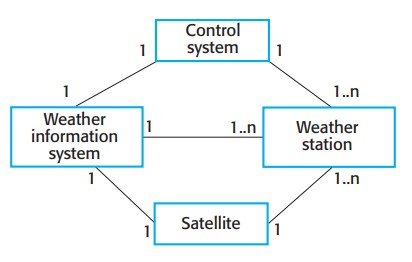
\includegraphics[scale=.5]{img/m3_1}
		\caption{System 
			context for the 
			weather station 
		}
	\end{figure}
	\column{.5\textwidth}
		\begin{figure}
		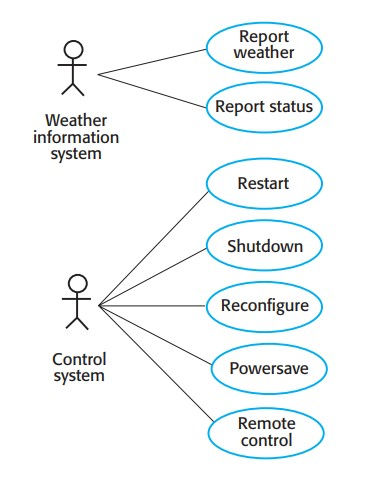
\includegraphics[scale=.5]{img/m3_2}
		\caption{Weather 
			station use cases
		}
	\end{figure}
\end{columns}
\end{frame}

\begin{frame}{Object-oriented design using the UML}
	%\textbf{System context and interactions}
		\begin{figure}
			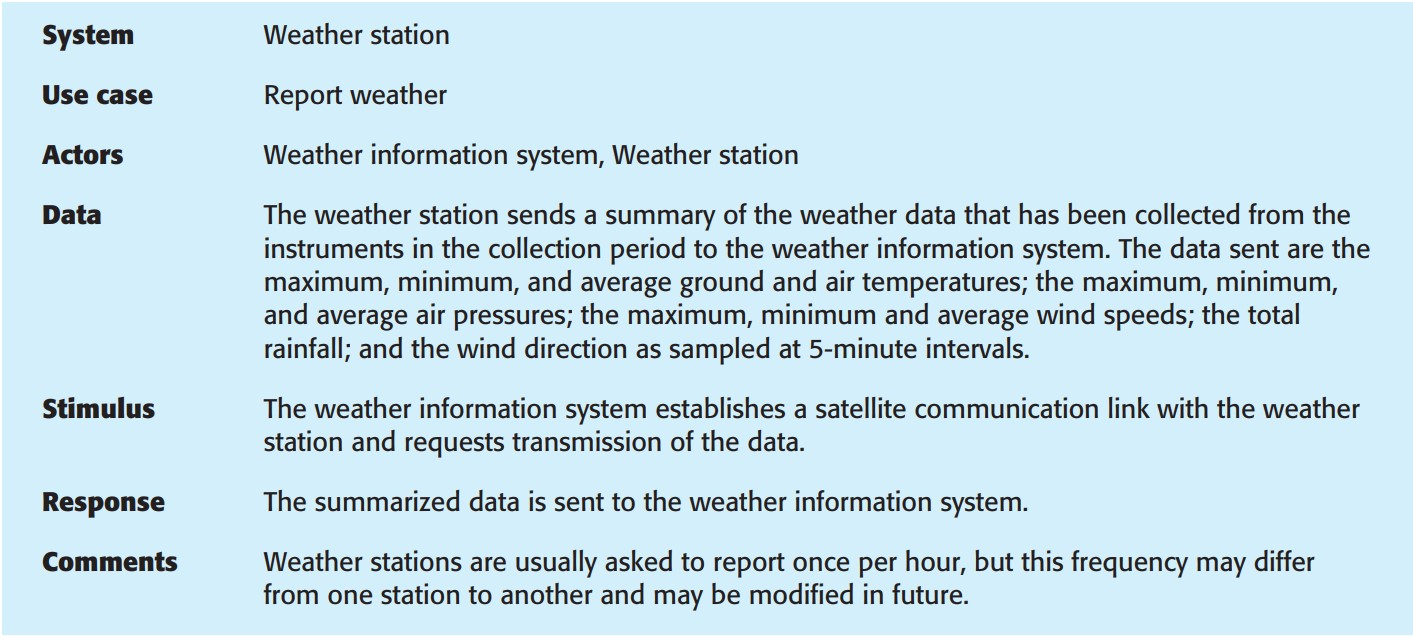
\includegraphics[scale=.4]{img/m3_3}
			\caption{Use case 
				description—Report 
				weathe
			}
		\end{figure}
\end{frame}

\begin{frame}{Object-oriented design using the UML}
	\textbf{Architectural Design:}
\begin{itemize}
	\item Once the interactions between the software system and the system’s 
	environment have been defined, you use this information as a basis 
	for designing the system architecture.
	\item \textbf{Identify the major components }that make up the system and their 
	interactions. 
	\item Then design the system organization using an architectural pattern 
	such as a layered or client–server model.

\end{itemize}
\end{frame}
\begin{frame}{Object-oriented design using the UML}
	%\textbf{System context and interactions}
	\begin{figure}
		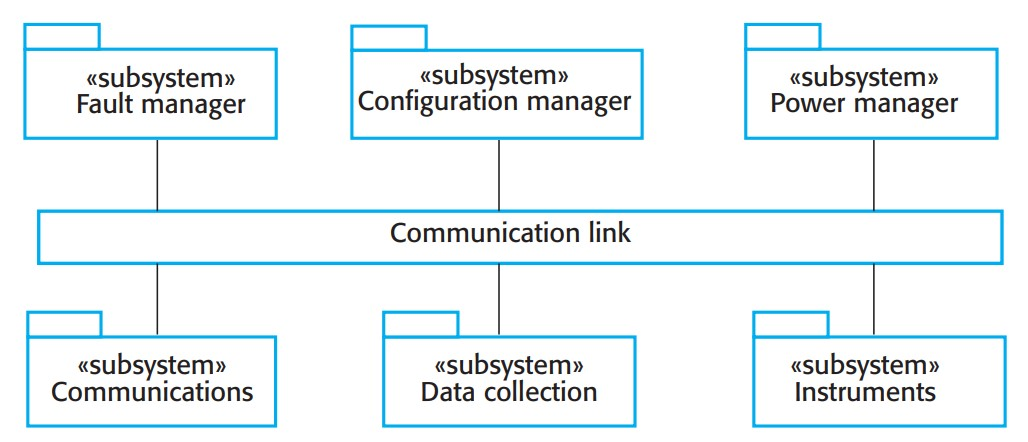
\includegraphics[scale=.5]{img/m3_4}
		\caption{High-level 
			architecture of 
			weather station 

		}
	\end{figure}
\end{frame}

\begin{frame}{Object-oriented design using the UML}
\textbf{Architectural Design Cont..}
\begin{itemize}
	\item The weather station is composed of independent subsystems that 
	communicate by broadcasting messages on a common infrastructure, 
	shown as Communication link in the figure.
	\item Each subsystem listens for messages on that infrastructure and picks 
	up the messages that are intended for them. This “listener model” is a 
	commonly used architectural style for distributed systems.
	\item The key benefit of this architecture is that it is easy to support 
	different configurations of subsystems because the sender of a 
	message does not need to address the message to a particular 
	subsystem.
\end{itemize}
\end{frame}
\begin{frame}{Object-oriented design using the UML}
	%\textbf{System context and interactions}
	\begin{figure}
		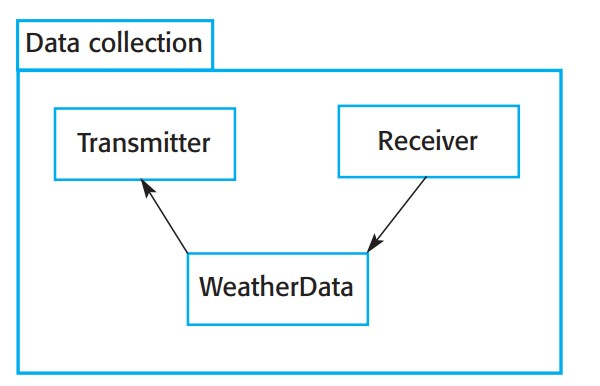
\includegraphics[scale=.5]{img/m3_5}
		\caption{Architecture 
			of data collection 
			system}
	\end{figure}
\end{frame}

\begin{frame}{Object-oriented design using the UML}
	\textbf{Object class identification}
	\begin{itemize}
	\item Identifying object classes is often a difficult part of object oriented design. There is no 'magic formula' for object identification.
\item  It relies on the skill, experience and domain knowledge of system designers.
	\item  Object identification is an iterative process. 
\item Various proposals are made to identify object 
classes in object oriented systems

	\begin{itemize}
		\item Use a \textbf{grammatical analysis approach} based on a natural language description of the 
		system. \begin{itemize}
			\item Eg:Objects and attributes are nouns; operations or services are verbs
		\end{itemize}
		\item Use \textbf{tangible entities (things)} in the application domain such as aircraft, roles such as 
		manager or doctor, events such as requests, interactions such as meetings, locations such 
		as offices, organizational units.
		\item Use a \textbf{scenario-based analysis} where various scenarios of system use are identified and 
		analysed and identify the required objects, attributes, and operations
	\end{itemize}
\end{itemize}
\end{frame}

\begin{frame}{Object-oriented design using the UML}
	\textbf{Object class identification}
	\begin{figure}
		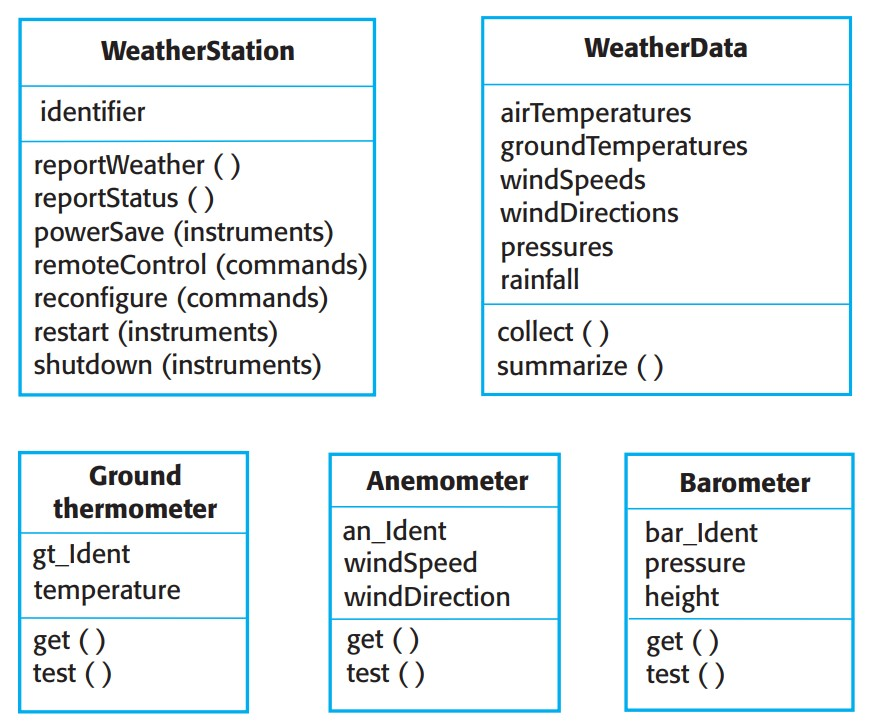
\includegraphics[scale=.4]{img/m3_6}
		\caption{Weather station objects}
	\end{figure}
\end{frame}
\begin{frame}{Object-oriented design using the UML}
	\textbf{Design models}
\begin{itemize}
	\item \textbf{Develop Design models} which \textbf{show the objects and object classes and relationships between these entities}. 
	\item When the UML is used to develop a design, two kinds of design models are normally 
	developed:

	\begin{itemize}
		\item \textbf{Structural models}, which describe the static structure of the system using object classes 
		and their relationships.
		\item \textbf{Dynamic models,} which describe the dynamic structure of the system and show the 
		interactions between the system objects.
		
	\end{itemize}
\item Examples of design models
\begin{itemize}
	\item \textbf{Subsystem models} that show logical groupings of 
	objects into coherent subsystems.
	\item \textbf{Sequence models} that show the sequence of object 
	interactions.
	\item \textbf{State machine models} that show how individual objects 
	change their state in response to events.
	\item Other models include \textbf{use-case models aggregation 
		models, generalisation models}, etc. ,
\end{itemize}
\end{itemize}
\end{frame}
\begin{frame}{Object-oriented design using the UML}
%	\textbf{Design models}
	\begin{figure}
	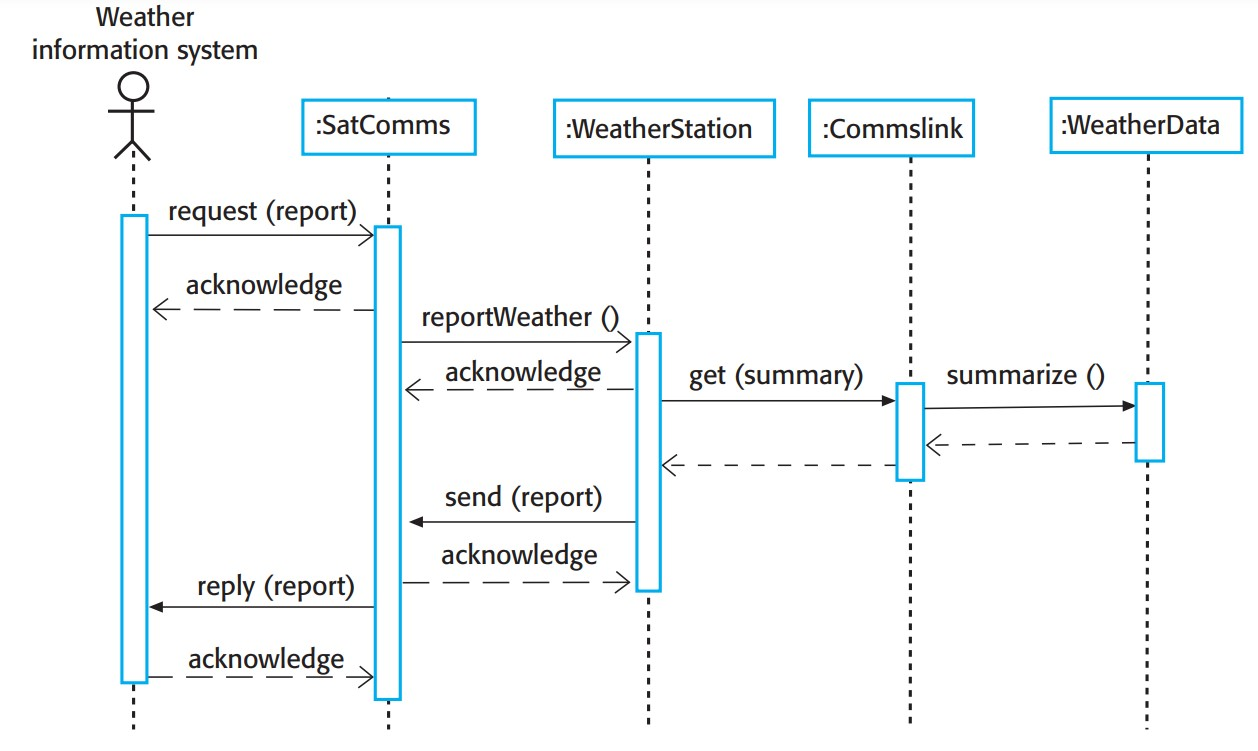
\includegraphics[scale=.4]{img/m3_7}
	\caption{Sequence 
		diagram describing 
		data collection
	}
\end{figure}
\end{frame}
\begin{frame}{Object-oriented design using the UML}
	%	\textbf{Design models}
	\begin{figure}
		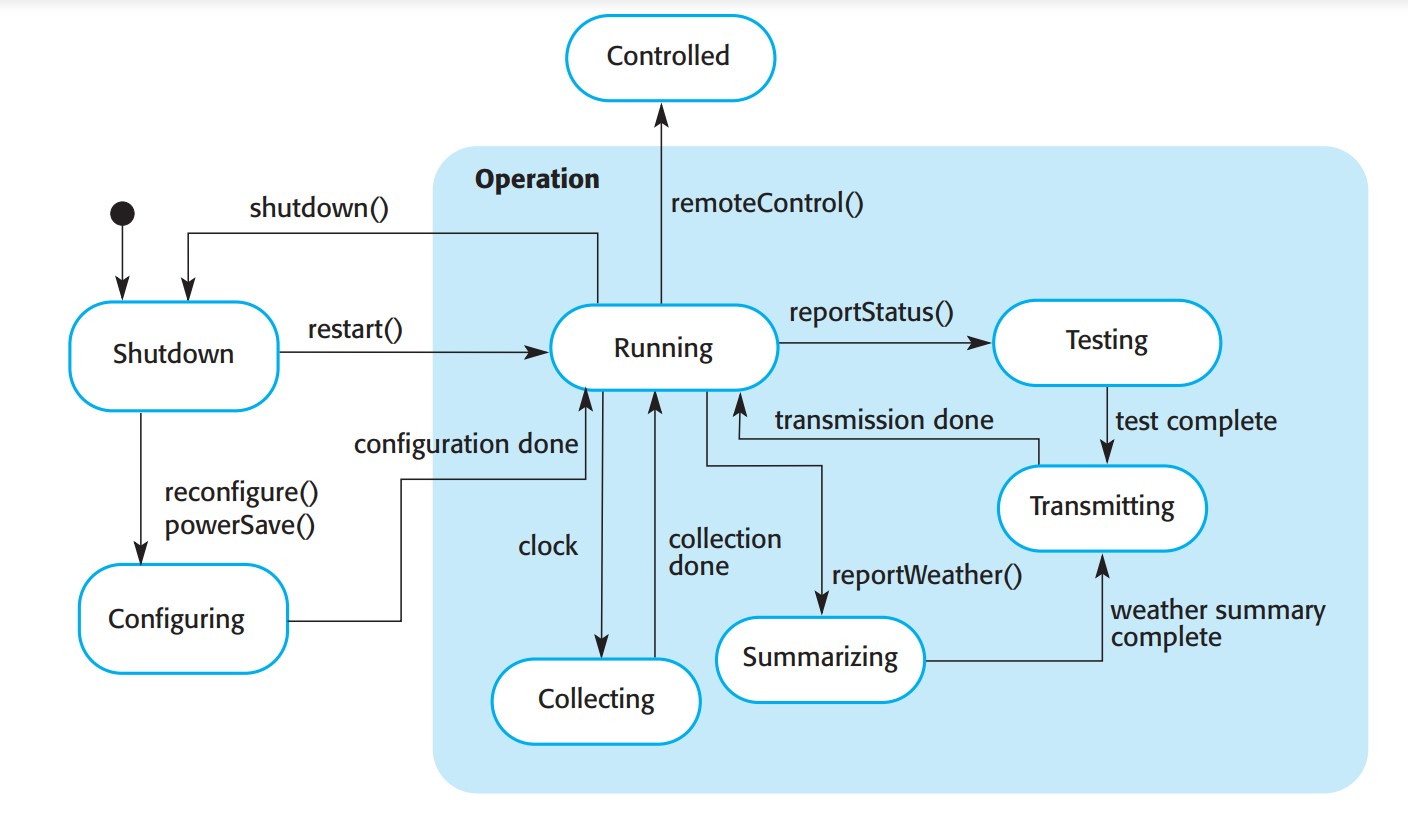
\includegraphics[scale=.4]{img/m3_8}
		\caption{Weather 
			station state diagram
		}
	\end{figure}
\end{frame}

\begin{frame}{Object-oriented design using the UML}
		\textbf{Interface specification}
		\begin{itemize}
			\item Interface design is concerned with specifying the detail of the interface to an object or to a group of objects
			\item Interfaces can be specified in the UML using the same notation as a class diagram. There 	is no attribute section and the UML stereotype $<<interface>>$ should be included in the 
			name part.
		\end{itemize}
		\begin{figure}
		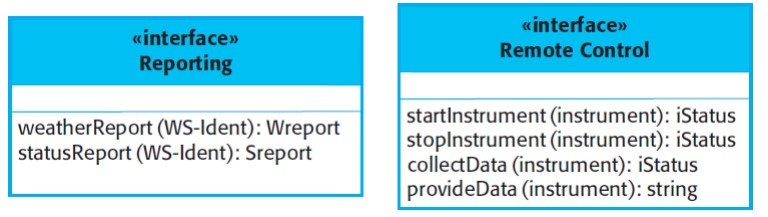
\includegraphics[scale=.5]{img/m3_9}
		\caption{Weather station interfaces
		}
	\end{figure}
\end{frame}
\section{Design Patterns}
\begin{frame}{Design Patterns}
	\textbf{{Design Patterns}}
\begin{itemize}
	\item A design pattern is a way of reusing abstract knowledge about a problem and its solution. 
	\item 
	\textbf{A pattern is a description of the problem and the essence of its solution. }It should be 
	sufficiently abstract to be reused in different settings.
	\item Pattern descriptions usually\textbf{ make use} of \textbf{object-oriented characteristics such as 
		inheritance and polymorphism}.

\item The four essential elements of design patterns
\begin{itemize}
	\item \textbf{Name}:A meaningful pattern identifier
	\item \textbf{Problem description}:A common situation where this pattern is applicable
	\item \textbf{Solution description}:Not a concrete design but a template for a design solution that can be instantiated in different ways
	\item \textbf{Consequences}:The results and trade-offs of applying the pattern

	

\end{itemize}
\end{itemize}

\end{frame}
\begin{frame}{Design Patterns}
	\begin{figure}
	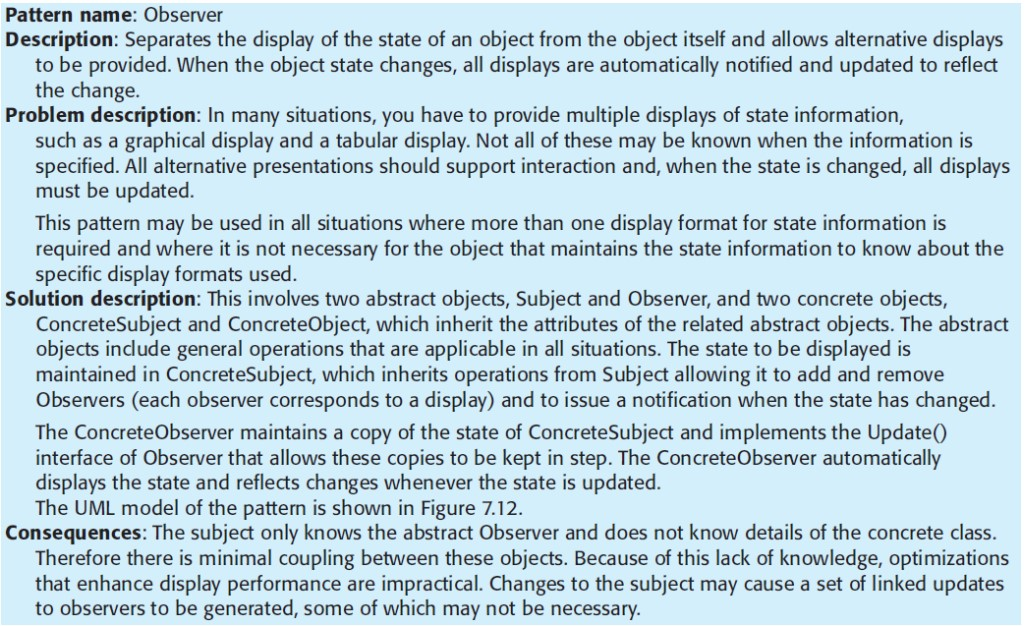
\includegraphics[scale=.5]{img/m3_11}
	\caption{The Observer pattern description.}
\end{figure}
	
\end{frame}
\begin{frame}{Design Patterns}
	\begin{figure}
		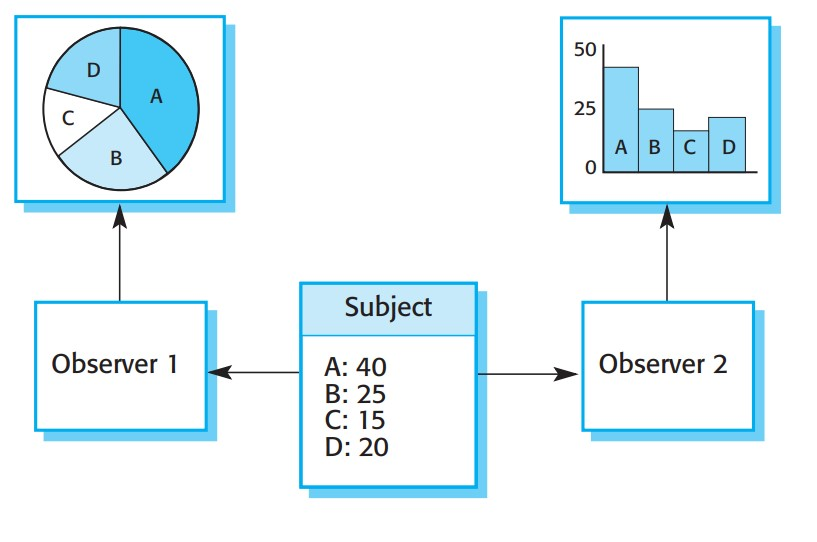
\includegraphics[scale=.5]{img/m3_10}
		\caption{The Observer pattern Graphical representation}
	\end{figure}
	
\end{frame}
\begin{frame}{Design Patterns}
	\begin{figure}
		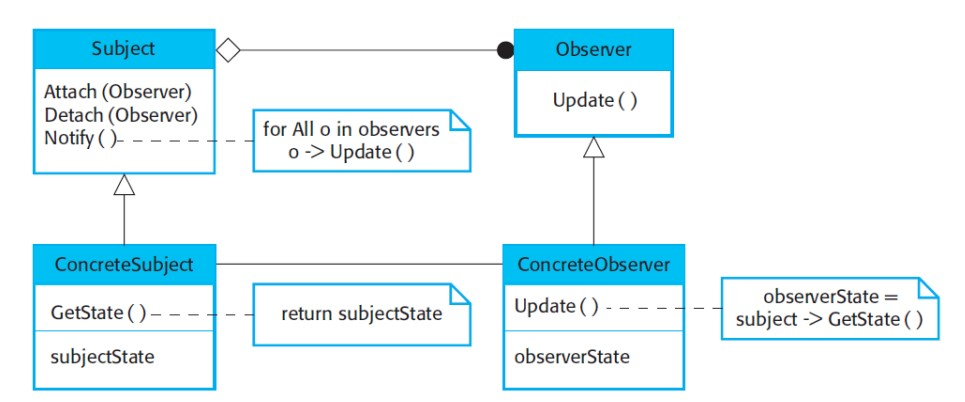
\includegraphics[scale=.5]{img/m3_12}
		\caption{A UML model of the Observer pattern}
	\end{figure}

\end{frame}

\begin{frame}{Design Patterns}
	\begin{itemize}
		\item There are four essential description elements and
		also include a brief statement of what the pattern can do.
		\item This pattern can be used in situations 
		where different presentations of an object’s state are required.
		\item Graphical representations are normally used to illustrate the object classes in patterns and their 
		relationships. 
		\item These supplement the pattern description and add detail to the solution 
		description.
	\end{itemize}
\end{frame}
\section{Implementation issues}
\begin{frame}{Implementation issues}
\textbf{Implementation issues}
\begin{itemize}
	\item Implementation is a critical stage where an executable version of the software is developed.
	\item Some of the aspects of implementation are:

	\begin{enumerate}
		\item Reuse
		\item Configuration management
		\item Host-target development
	\end{enumerate}
\end{itemize}
\end{frame}
\begin{frame}{Implementation issues}
	\begin{itemize}
		\item[1] \textbf{Reuse}
		\begin{itemize}
			\item Most modern software is constructed by reusing existing components or 
			systems. 
			\item When developing software, make use of existing code as much as possible.
			
			\item Software reuse is possible at a number of different levels:
			\begin{itemize}
				\item \textbf{The abstraction level:} don't reuse software directly but use knowledge of successful abstractions in the software design.
				\item \textbf{The object level:} directly reuse objects from a library rather than writing the code yourself.
				\item \textbf{The component level:} components (collections of objects and object classes) are reused in application systems.
				\item \textbf{The system level:} entire application systems are reused.
			\end{itemize}
		\end{itemize} 
	\end{itemize}
\end{frame}

\begin{frame}{Implementation issues}
	\begin{figure}
	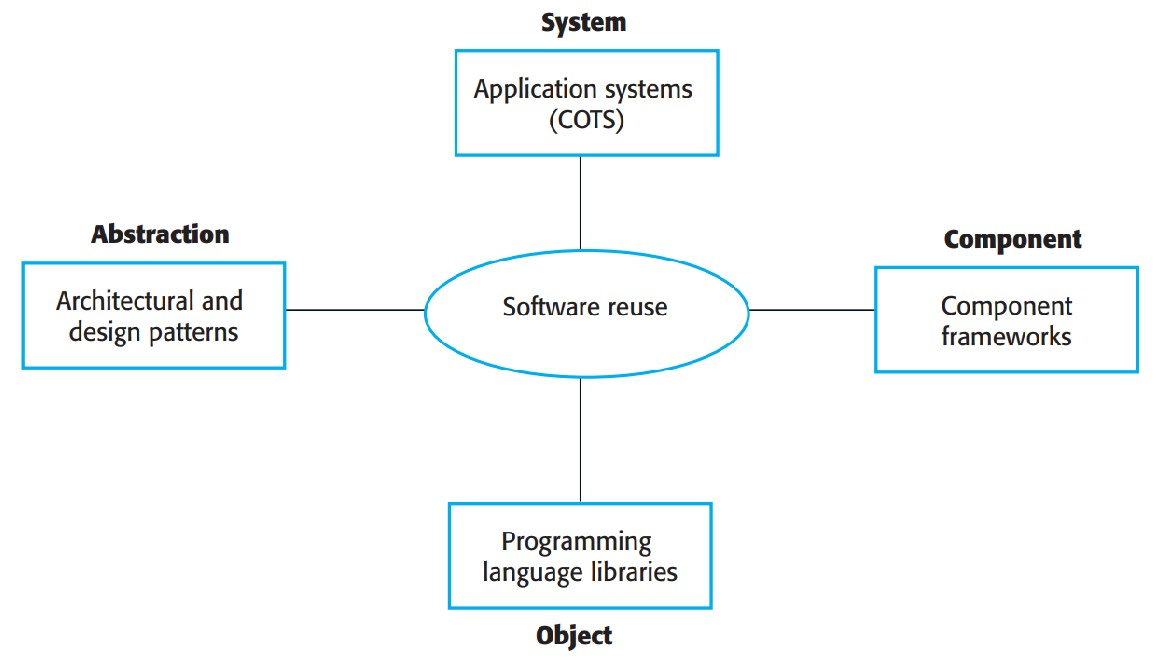
\includegraphics[scale=.45]{img/m3_13}
	\caption{Software 
		reuse
	}
\end{figure}

\end{frame}
\begin{frame}{Implementation issues}
\textbf{Costs of reuse:}
\begin{itemize}
	\item The costs of the\textbf{ time }spent in looking for software to reuse and assessing whether or not it meets your needs.
	\item Where applicable, the costs of\textbf{ buying }the reusable software. For large off-the-shelf systems, these costs can be very high.
	\item The costs of \textbf{adapting and configuring} the reusable software components or systems to reflect the requirements of the system that you are developing.
	\item The costs of\textbf{ integrating} reusable software elements with each other (if you are using software from different sources) and with the new code that you have developed.
\end{itemize}
\end{frame}
\begin{frame}{Implementation issues}
\begin{itemize}
	\item[2] \textbf{Configuration management}
	\begin{itemize}
		\item Configuration management is the name given to the general \textbf{process of managing a 
			changing software system. }
		\item The aim of configuration management is to support the system integration process so 
		that all developers can access the project code and documents in a controlled way, find 
		out what changes have been made, and compile and link components to create a system.
	\end{itemize} 
\end{itemize}
\end{frame}
\begin{frame}{Implementation issues}
	\textbf{There are three fundamental configuration management activities:}
	\begin{itemize}
		\item \textbf{Version management:} where support is provided to keep track of the different versions 
		of software components. Version management systems include facilities to coordinate 
		development by several programmers.
		\item \textbf{System integration:} where support is provided to help developers define what versions 
		of components are used to create each version of a system. This description is then used 
		to build a system automatically by compiling and linking the required components.
		\item \textbf{Problem tracking:} where support is provided to allow users to report bugs and other 
		problems, and to allow all developers to see who is working on these problems and when 
		they are fixed.
		
	\end{itemize}
\end{frame}

\begin{frame}{Implementation issues}
	\begin{figure}
		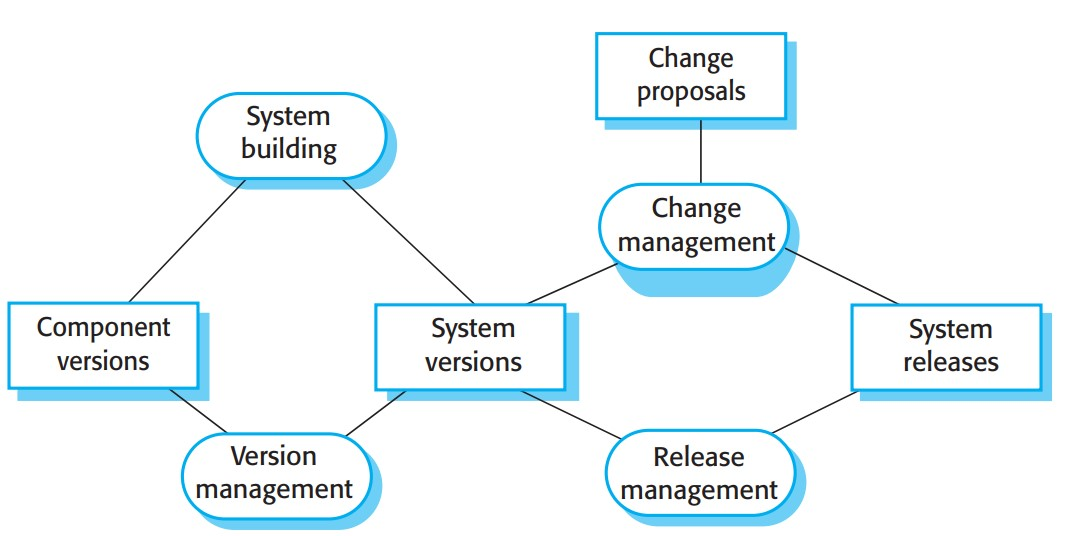
\includegraphics[scale=.45]{img/m3_14}
		\caption{Configuration 
			management}
	\end{figure}
	
\end{frame}

\begin{frame}{Implementation issues}
\begin{itemize}
	\item[3] \textbf{Host-target development}
	\begin{itemize}
		\item Most software is developed on one computer (the host, development platform), but runs on a separate machine (the target, execution platform). 
		\item A platform is more than just hardware; it includes the installed operating system plus other supporting software such as a database management system or, for development platforms, an interactive development environment (IDE). 
		\item Development platform usually has different installed software than execution platform; these platforms may have different architectures. 
		\item Mobile app development (e.g. for Android) is a good example.
		
	\end{itemize} 
\end{itemize}
\end{frame}
\begin{frame}{Implementation issues}
	\textbf{A software development platform should provide a range of tools to 
		support software engineering processes. These may include:}
	\begin{itemize}
		\item An integrated compiler and syntax-directed editing system that allows you to 
		create, edit, and compile code.
		\item A language debugging system.
		\item Graphical editing tools, such as tools to edit UML models.
		\item Testing tools, such as JUnit that can automatically run a set of tests on a new version of a program.
		\item Tools to support refactoring and program visualization
		\item Configuration management tools to manage source code versions and to integrate 
		and build systems.
		
	\end{itemize}
\end{frame}
\begin{frame}{Implementation issues}
	\begin{figure}
		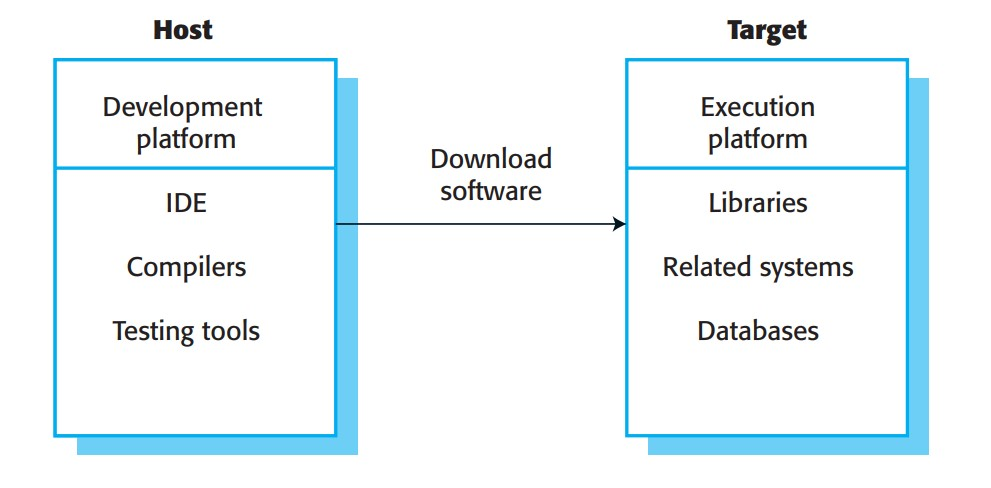
\includegraphics[scale=.45]{img/m3_15}
		\caption{Host-target 
			development}
	\end{figure}
	
\end{frame}
\section{Open source development}
\begin{frame}{Open source development}
\textbf{Open source development}
\begin{itemize}
	\item  Open-source development is an approach to software development 
	in which the \textbf{source code of a software system is published }and 
	volunteers are invited to participate in the development process.

	\item Its roots are in the Free Software Foundation 
	(www.fsf.org), which advocates that source code should 
	not be proprietary but rather should always be available 
	for users to examine and modify as they wish. 

	\item The best-known open source product is, of course, the 
	Linux operating system which is widely used as a server 
	system and, increasingly, as a desktop environment.
	\item Other important open source products are Java, the 
	Apache web server and the mySQL database 
	management system. 
	\item A fundamental principle of open-source development is 
	that source code should be freely available, this does not 
	mean that anyone can do as they wish with that code.
\end{itemize}
\end{frame}
\begin{frame}{Open source development}
	\textbf{Open source development:Typical licensing models include:}
	\begin{itemize}
		\item  The \textbf{GNU General Public License (GPL)}. This is a so-called 'reciprocal' license that means that \textbf{if you use }open source software that is licensed under the GPL license, then \textbf{you must make that software open source}.
		\item The GNU\textbf{ Lesser General Public License (LGPL)} is a variant of the GPL license where \textbf{you can write components that link to open source code without having to publish the source }of these components.
		\item The\textbf{ Berkley Standard Distribution (BSD)} License. This is a non-reciprocal license, which means you are not obliged to re-publish any changes or modifications made to open source code. You can include the code in proprietar
		y systems that are sold.
	\end{itemize}
\end{frame}
\section{Review Techniques}
\begin{frame}{Review Techniques}
\textbf{Review Techniques}
\begin{itemize}
	\item Software reviews are a “filter” for the software process.
	\item \textbf{Reviews are applied at various points during software engineering and serve to uncover errors and defects that can then be removed. }
	\item Software reviews “purify” software engineering work products, 
	including requirements and design models, code, and testing data.
	\item A review—any review—is a way of using the diversity of a group of 
	people to
	\begin{itemize}
		\item \textbf{Point out needed improvements} in the product of a single 
		person or team;
		\item \textbf{Confirm those parts} of a product in which \textbf{improvement is 
			either not desired or not needed;}
	\end{itemize}

\end{itemize}
\end{frame}
\begin{frame}{Review Techniques}
	\textbf{Cost impact of Software Defects}
	\begin{itemize}
		\item Within the context of the software process, the terms defect and fault are synonymous.
		\item Both imply a quality problem that is discovered after the software has been released to end users.
		
		\item \textbf{The primary objective of technical reviews is to find errors during the process so that they do not become defects after release of the software. }
		\item The obvious benefit of technical reviews is the early discovery of errors so that they do not
		propagate to the next step in the software process.
		\item \textbf{Review techniques have been shown to be up to 75 percent effective in 
			uncovering design flaws.}
		\item By\textbf{ detecting and removing} a large percentage of these errors, the review process substantially \textbf{reduces the cost of subsequent activities in the software process.}
		
	\end{itemize}
\end{frame}

\begin{frame}{Review Techniques}
	\textbf{DEFECT AMPLIFICATION AND REMOVAL}
	\begin{itemize}
		\item A defect amplification model can be used to \textbf{illustrate the generation and detection of errors during the design and code generation actions of a software process}. 
		\item To conduct reviews, you must expend time and effort, and your development 
		organization must spend money
		
	\end{itemize}

\end{frame}
\begin{frame}{Review Techniques}
%	\textbf{DEFECT AMPLIFICATION AND REMOVAL}
	\begin{itemize}
		\item A box represents a software engineering action. 
		During the action, errors may be inadvertently generated. 
		\item Review may fail to uncover newly generated errors and errors from previous steps, resulting in some number of errors that are passed through. 
		\item In some cases, errors passed through from previous steps are amplified (amplification factor, x ) by current work. 
		\item The box subdivisions represent each of these characteristics and the percent of efficiency for detecting errors, a function of the thoroughness of the review.
		
	\end{itemize}
	\begin{figure}
		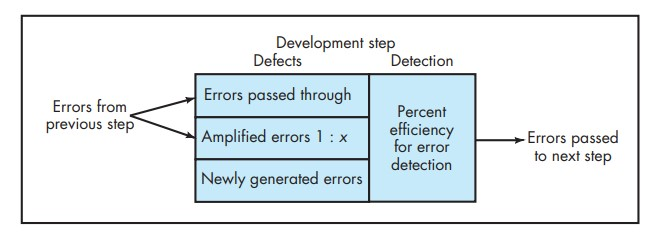
\includegraphics[scale=.45]{img/m3_16}
		\caption{Defect 
			amplifi cation 
			model}
	\end{figure}
\end{frame}
\begin{frame}{Review Techniques}
%	\textbf{DEFECT AMPLIFICATION AND REMOVAL}
	\begin{itemize}
		\item Referring to the figure, each test step is assumed to uncover and correct 50 percent of all   incoming errors without introducing any new errors (an optimistic assumption). 
		\item Ten preliminary design defects are amplified to 94 errors before testing commences. 
		\item Twelve latent errors are released to the field
		
	\end{itemize}
	\begin{figure}
		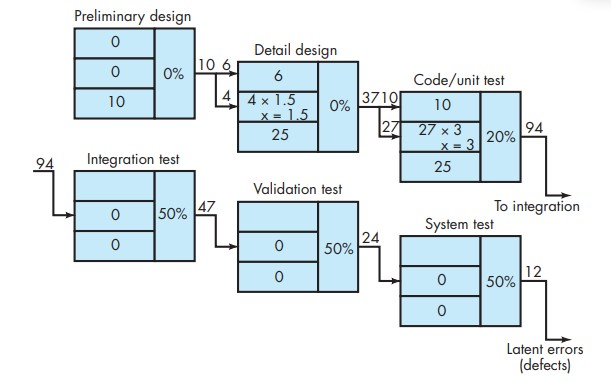
\includegraphics[scale=.5]{img/m3_17}
		\caption{Defect 
			amplifi cation—
			no reviews}
	\end{figure}
\end{frame}
\begin{frame}{Review Techniques}
%	\textbf{DEFECT AMPLIFICATION AND REMOVAL}
	\begin{itemize}
		\item In this case, 10 initial preliminary (architectural) design errors are amplified to 24 errors before testing commences. 
		\item Only three latent errors exist. 
		\item The relative costs associated with the discovery and correction of errors, overall cost (with and without review for our hypothetical example) can be established.
		
		
	\end{itemize}
	\begin{figure}
		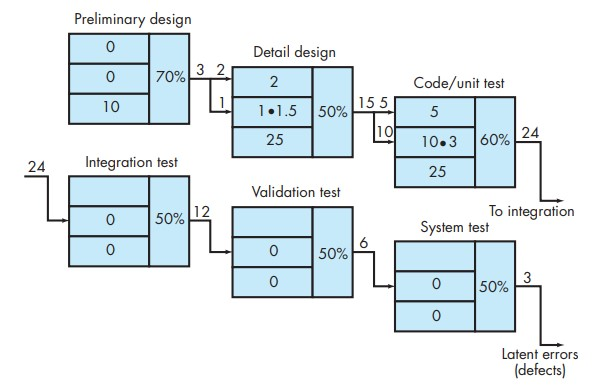
\includegraphics[scale=.5]{img/m3_18}
		\caption{Defect 
			amplifi cation—
			reviews 
			conducted}
	\end{figure}
\end{frame}
\begin{frame}{Review Techniques}
	%	\textbf{DEFECT AMPLIFICATION AND REMOVAL}
	\begin{itemize}
		\item Using these data, the total cost for development and maintenance when reviews are conducted is 783 cost units. 
		\item When no reviews are conducted, total cost is 2177 units—nearly three times more costly.
		
	\end{itemize}
\end{frame}
\begin{frame}{Review Techniques}
		\textbf{REVIEW METRICS AND THEIR USE}
	\begin{itemize}
		\item Technical reviews are one of many actions that are required as part of good software engineering practice. 
		\item Each action requires dedicated human effort. 
		\item Since available project effort is finite, it is important for a software engineering organization   to understand the effectiveness of each action by defining a set of metrics that can be used to assess their efficacy.
		\item Although many metrics can be defined for technical reviews, a relatively small subset can provide useful insight. 
		
		
	\end{itemize}
\end{frame}
\begin{frame}{Review Techniques}
	\textbf{The following review metrics can be collected for each review that is conducted:
	}
	\begin{itemize}
		\item \textbf{Preparation effort, $E_p$} —the effort (in person-hours) required to review a work product prior to  the actual review meeting
		\item \textbf{Assessment effort, $E_a$} — the effort (in person-hours) that is expended during the actual review
		\item \textbf{Rework effort, $E_r$ }— the effort (in person-hours) that is dedicated to the correction of those errors uncovered during the review
		\item \textbf{Work product size, WPS} —a measure of the size of the work product that has been reviewed (e.g., the number of UML models, or the number of document pages, or the number of lines of code)
	\item \textbf{Minor errors found, $Err_{minor}$} —the number of errors found that can be categorized as minor (requiring less than some prespecified effort to correct)
		\item \textbf{Major errors found, $Err_{major}$} —the number of errors found that can be categorized as major (requiring more than some prespecified effort to correct)
		
	\end{itemize}
\end{frame}
\begin{frame}{Review Techniques}
	\textbf{ANALYZING MATRICES}
	\begin{itemize}
	
		\item The total review effort and the total number of errors discovered are defi ned as:
		$$Ereview = Ep + Ea + Er$$ $$ Errtot = Errminor + Errmajor$$
		\item Error density represents the errors found per unit of work product reviewed.
		$$Error density = Errtot/ WPS$$
	\end{itemize}
\end{frame}
\begin{frame}{Review Techniques}
	\textbf{Cost-Effectiveness of Reviews}
	\begin{itemize}
		\item It is difficult to measure the cost-effectiveness of any technical review in real time.
		\item A software engineering organization can assess the effectiveness of reviews and their cost benefit only after reviews have been completed, \textbf{review metrics have been collected, average data have been computed, and   then the downstream quality of the software is measured}
		$$ Effort saved per error = Etesting - Ereviews $$
	\end{itemize}
\end{frame}
\begin{frame}{Review Techniques}
	\textbf{Effort expended with and without reviews}
	\begin{itemize}
		\item Effort expended when reviews are used does increase early in the development of a software increment. 
		\item Testing and corrective effort is reduced. 
		\item The deployment date for development with reviews is sooner than the deployment date without reviews. 
		\item Reviews don’t take time, they save it. 
			\begin{figure}
			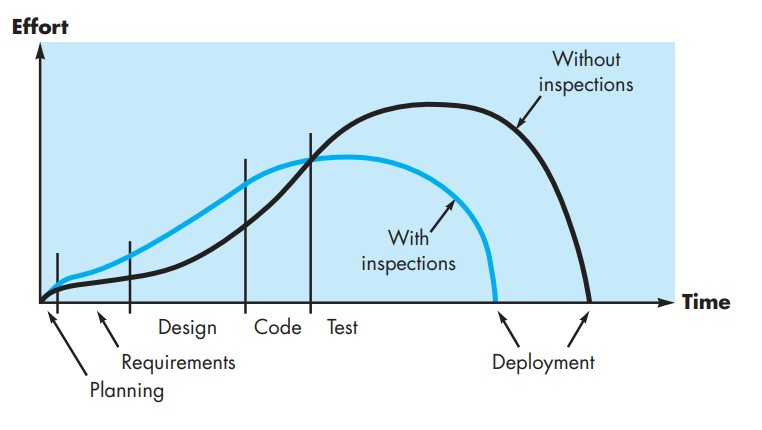
\includegraphics[scale=.4]{img/m3_19}
			\caption{Effort expended with and without 	reviews}
		\end{figure}
	\end{itemize}
\end{frame}
\begin{frame}{Review Techniques}
	\textbf{CODE REVIEWS}
	\begin{itemize}
		\item\textbf{ Code reviews that focus on security issues should be included as part of the implementation activities. }
		\item These code reviews should be based on the appropriate security objectives and threats identified in the        system design activities.
		\item Code reviews are known to \textbf{reduce the number of product defects prior to testing}, which in turn \textbf{eliminates   potential security holes and improves software quality}.
		
	\end{itemize}
	\begin{figure}
	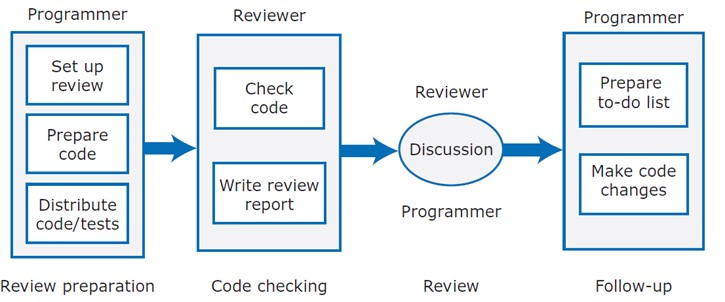
\includegraphics[scale=.4]{img/m3_20}
	%\caption{Effort expended with and without 	reviews}
\end{figure}
\end{frame}
\begin{frame}{Review Techniques}
	\textbf{Code review activities}
	\begin{figure}
		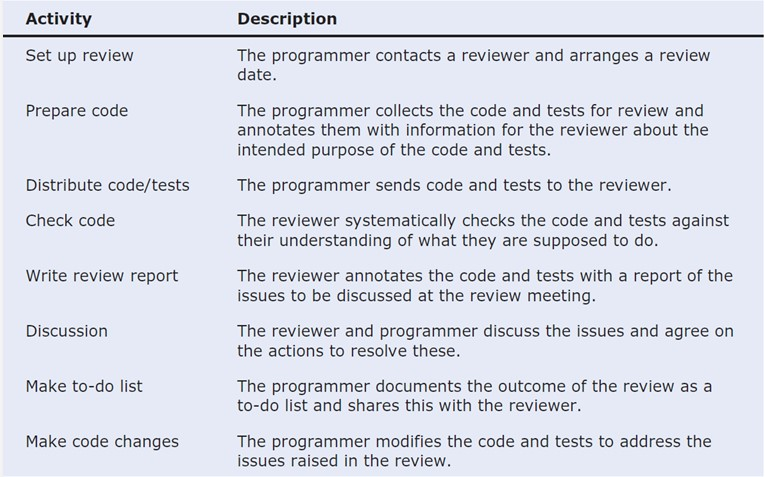
\includegraphics[scale=.7]{img/m3_21}
		%\caption{Effort expended with and without 	reviews}
	\end{figure}
\end{frame}
\begin{frame}{Review Techniques}
\textbf{REVIEWS : A FORMALITY SPECTRUM}
\begin{itemize}
	\item Technical reviews should be applied with a level of formality that is 
	appropriate for the product to be built, the project time line, and the 
	people who are doing the work.
	\item The formality of a review increases when
	\begin{itemize}
		\item Distinct roles are explicitly defined for the reviewers,
		\item There is a sufficient amount of planning and preparation for 
		the review,
		\item A distinct structure for the review (including tasks and internal 
		work products) is defined
		\item A set of specific tasks would be conducted based on 
		an agenda that was developed before the review 
		occurred. 
		\item The results of the review would be formally 
		recorded, and the team would decide on the status of 
		the work product based on the outcome of the review.
		\item Members of the review team might also verify that 
		the corrections made were done properly
		
	\end{itemize}
\end{itemize}
\end{frame}
\begin{frame}{Review Techniques}
	\textbf{REVIEWS : A FORMALITY SPECTRUM cont..}
		\begin{figure}
		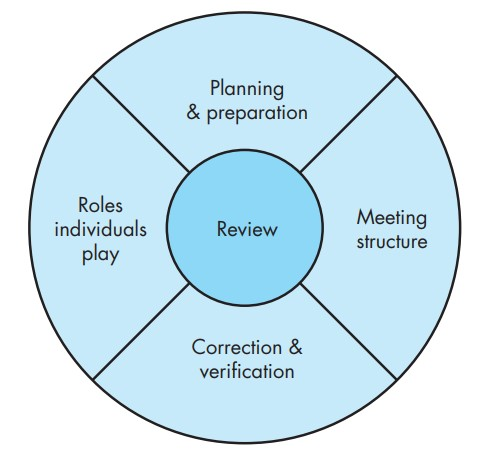
\includegraphics[scale=.4]{img/m3_22}
		\caption{Reference 
			model for 
			technical 
			reviews}
	\end{figure}
\end{frame}
\begin{frame}{Review Techniques}
	\textbf{Technical reviews:}
	\begin{itemize}
		\item Informal reviews
		\item Formal technical reviews. 
		
	\end{itemize}
	
\end{frame}
\begin{frame}{Review Techniques}
	\textbf{Informal reviews:}
	\begin{itemize}
		\item Informal reviews \textbf{include a simple desk check of a software engineering work product with 
			a colleague, a casual meeting }(involving more than two people) for the purpose of 
		reviewing a work product.
		\item One way to\textbf{ improve the efficacy of a desk check review} is to\textbf{ develop 
			a set of simple review checklists for each major work product }
		produced by the software team.
		\item Checklist for interfaces
		\begin{itemize}
			\item Is the layout designed using standard conventions? Left to right? Top 
			to bottom? 
		\item Does the presentation need to be scrolled? 
			\item Are color and placement, typeface, and size used effectively?
			\item Are all navigation options or functions represented at the same level of 
			abstraction? 
			\item Are all navigation choices clearly labeled?
		\end{itemize}
		
	\end{itemize}
	
\end{frame}
\begin{frame}{Review Techniques}
	\textbf{Informal reviews Cont...}
	\begin{itemize}
		\item Any errors or issues noted by the reviewers are recorded by the designer 
		for resolution at a later time
		\item \textbf{Pair programming} can be characterized as a continuous desk check. 
		Rather than scheduling a review at some point in time
		\item Pair programming encourages continuous review as a work product 
		(design or code) is created. 
		\item The benefit is immediate discovery of errors and better work product 
		quality as a consequence.
	\end{itemize}
	
\end{frame}
\begin{frame}{Review Techniques}
	\textbf{FORMAL TECHNICAL REVIEWS}
	\begin{itemize}
		\item  A formal technical review (FTR) is a \textbf{software quality control activity performed by software engineers }(and others).
		\item The objectives of an FTR are:
		\begin{itemize}
			\item \textbf{To uncover errors in function, logic, or implementation} for any 
			representation of the software;
			\item \textbf{To verify that the software} under review \textbf{meets its requirements; }
			\item  \textbf{To ensure that the software has been represented according to predefined 
				standards;}
			\item \textbf{To achieve software that is developed in a uniform manner;} and
			\item To\textbf{ make projects more manageable}
		\end{itemize}
	\end{itemize}
\end{frame}

\begin{frame}{Review Techniques}
	\textbf{FORMAL TECHNICAL REVIEWS Cont..}
	\begin{itemize}
		\item FTR serves as a training ground, enabling junior engineers to observe 
		different approaches to software analysis, design, and implementation.
		\item The FTR also serves to promote backup and continuity because a 
		number of people become familiar with parts of the software that they 
		may not have otherwise seen.
		\item The FTR is actually a class of reviews that includes walkthroughs and 
		inspections.
		\item Each FTR is conducted as a meeting and will be successful only if it is 
		properly planned, controlled, and attended.
	\end{itemize}
\end{frame}
\begin{frame}{Review Techniques}
\textbf{FORMAL TECHNICAL REVIEWS}
\begin{itemize}
	\item The Review Meeting
	\item Review Reporting and Record Keeping
	\item Review Guidelines
\end{itemize}
\end{frame}


\begin{frame}{FORMAL TECHNICAL REVIEWS}
	\textbf{$[1]$.The Review Meeting}
	\begin{itemize}
		\item Regardless of the FTR format that is chosen, every review meeting should abide 
		by the following constraints:
		\begin{itemize}
			\item Between \textbf{three and five people} (typically) should be \textbf{involved} in the 
			review.
			\item \textbf{Advance preparation should occur} but should require no more than 
			two hours of work for each person.
			\item The duration of the review meeting should be \textbf{less than two hours.}
		\end{itemize}
	\item The \textbf{focus }of the FTR is \textbf{on a work product} (e.g., a portion of a 
	requirements model, a detailed component design, source code for a 
	component).
	\end{itemize}
\end{frame}
\begin{frame}{FORMAL TECHNICAL REVIEWS}
	\textbf{The Review Meeting cont..}
	\begin{itemize}
		\item The individual who has developed the work product—\textbf{the producer—
			informs the project leader that the work product is complete and that 
			a review is required.}
		\item Each reviewer is \textbf{expected to spend between one and two hours 
			reviewing the product, making notes.}
		\item The review meeting is \textbf{attended by the review leader, all reviewers, 
			and the producer}
		\item \textbf{One of the reviewers takes on the role of a recorder,} that is, the 
		individual who records (in writing) all important issues raised during 
		the review.
	
	\end{itemize}
\end{frame}

\begin{frame}{FORMAL TECHNICAL REVIEWS}
	\textbf{The Review Meeting cont..}
	\begin{itemize}

		\item The FTR \textbf{begins with an introduction of the agenda and a brief 
			introduction by the producer.}
		\item The producer \textbf{then proceeds to “walk through” }the work product, 
		explaining the material, while reviewers raise issues based on their 
		advance preparation. When valid problems or errors are discovered, 
		the recorder notes each.
		\item \textbf{At the end }of the review, all attendees of the FTR must decide whether to:
		\begin{itemize}
			\item \textbf{accept }the product \textbf{without further modification,}
			\item \textbf{reject the product} due to severe errors (once corrected, another review 
			must be performed), or

			\item \textbf{ accept the product provisionally }(minor errors have been encountered 
			and must be corrected, but no additional review will be required).
		\end{itemize}
	\item After the decision is made, all FTR\textbf{ attendees complete a sign-off, indicating 
		their participation} in the review and their concurrence with the review 
	team’s findings.
	\end{itemize}
\end{frame}

\begin{frame}{FORMAL TECHNICAL REVIEWS}
	\textbf{[2]. Review Reporting and Record Keeping}
	\begin{itemize}
		\item During the FTR, a \textbf{reviewer (the recorder) actively records all issues 
			that have been raised.}
		\item These are \textbf{summarized at the end} of the review meeting, and a review 
		\textbf{issues list is produced}
		\item In addition, a formal technical review summary report is completed.
		\item A review \textbf{summary report answers three questions:}
		\begin{itemize}
			\item What was reviewed? 
			\item Who reviewed it? 
			\item What were the findings and conclusions?
			
		\end{itemize}
	\end{itemize}
\end{frame}

\begin{frame}{FORMAL TECHNICAL REVIEWS}
	\textbf{ Review Reporting and Record Keeping cont..}
	\begin{itemize}
		\item The review issues list serves two purposes:
		\begin{itemize}
			\item to \textbf{identify problem areas} within the product and
			\item to serve as an action item \textbf{checklist that guides the producer as corrections are made. }
		\end{itemize}
	\item An issues list is normally attached to the summary report.
	\end{itemize}
\end{frame}
\begin{frame}{FORMAL TECHNICAL REVIEWS}
	\textbf{[3.] Review Guidelines}
	\begin{itemize}
		\item Minimum set of guidelines for formal technical reviews:
		\begin{enumerate}
			\item Review the product, not the producer
			\item Set an agenda and maintain it. 
			\item Limit debate and rebuttal. 
			\item Enunciate problem areas, but don't attempt to solve every problem noted.. 
			\item Take written notes. 
		\item Limit the number of participants and insist upon advance preparation. 
			\item Develop a checklist for each product that is likely to be reviewed. 
		\item Allocate resources and schedule time for FTRs..
		\item  Conduct meaningful training for all reviewers. 
			\item Review your early reviews
			
		\end{enumerate}
	\end{itemize}
\end{frame}

\begin{frame}{POST-MORTEM EVALUATIONS}
\textbf{POST-MORTEM EVALUATIONS(PME)}
\begin{itemize}
	\item Post-mortem evaluation (PME) as a \textbf{mechanism to determine what went right and what 
		went wrong }when software engineering process and practice are applied in a specific 
	project. 
	\item Unlike an FTR that focuses on a specific work product, a\textbf{ PME 
		examines} the entire software project, focusing on both \textbf{“ excellences 
		and challenges”} a PME is attended by members of the software team 
	and stakeholders.
	\item The intent is to\textbf{ identify excellences and challenges} and to \textbf{extract 
		lessons learned from both}. 
	\item The objective is to\textbf{ suggest improvements to both process and practice }
	going forward
\end{itemize}
\end{frame}
\section{Software testing strategies}
\begin{frame}{Software testing strategies}
\textbf{Software testing strategies}
\begin{itemize}
	\item Testing is a set of activities that can be planned in advance and conducted systematically.
	\item Any testing strategy must incorporate,
	\begin{itemize}
		\item Test planning
		\item Test-case design
		\item Test execution
		\item Resultant data collection and evaluation.
	\end{itemize}
\end{itemize}
\end{frame}
\begin{frame}{Software testing strategies}
	\textbf{Characteristics of software testing strategies}
	\begin{itemize}
		\item \textbf{To perform effective testing}, you should \textbf{conduct effective technical reviews} . By doing 
		this, many errors will be eliminated before testing commences.
		\item Testing \textbf{begins at the component level} and \textbf{works “outward” toward the integration of the 
			entire computer-based system}.
		\item \textbf{Different testing techniques} are appropriate \textbf{for different software engineering approaches }
		and \textbf{at different points in time.}
		\item Testing is \textbf{conducted by the developer} of the software \textbf{and} (for large projects) \textbf{an independent test group.}
		\item \textbf{Testing and debugging are different activities}, but debugging must be accommodated in 
		any testing strategy.
	\end{itemize}
\end{frame}
\begin{frame}{Software testing strategies}
	\textbf{Verification and Validation}
	\begin{itemize}
		\item \textbf{Verification} refers to the set of tasks that\textbf{ ensure that software correctly implements a specific function. }
		\item \textbf{Validation} refers to a different set of tasks that \textbf{ensure that the software that has     been built is traceable to customer requirements. }
		\item Boehm states this another way:
		\begin{itemize}
			\item \textbf{Verification:} \emph{ “Are we building the product right?”}
			\item \textbf{Validation:} \emph{ “Are we building the right product?”}
		\end{itemize}
	\end{itemize}
\end{frame}
\begin{frame}{Software testing strategies}
		\begin{figure}
	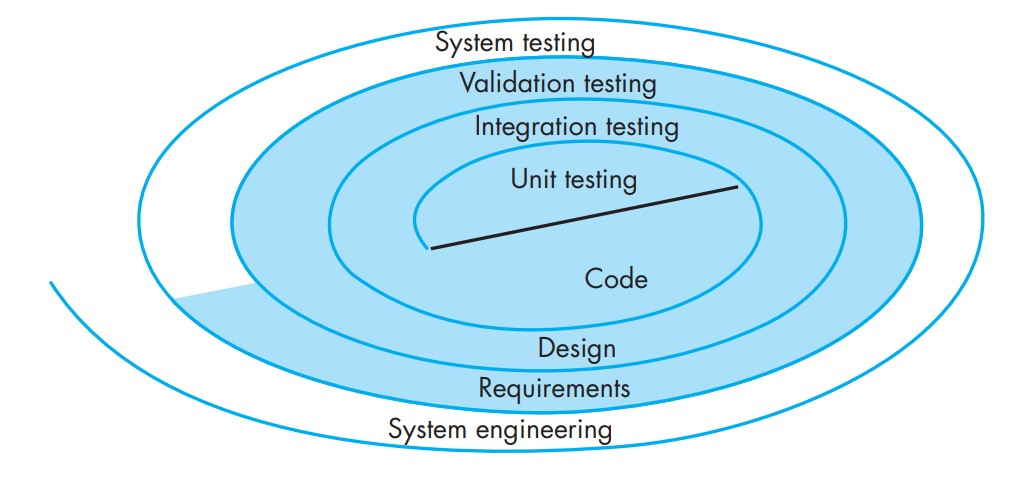
\includegraphics[scale=.5]{img/m3_23}
	\caption{Testing 
		strategy}
\end{figure}
\end{frame}
\begin{frame}{Software testing strategies}
\begin{enumerate}
	\item UNIT TESTING
	\begin{itemize}
		\item 	Unit Test Considerations
	\end{itemize}
	\item INTEGRATION TESTING
	\begin{enumerate}[i]
		\item Top-Down Integration
		\item Bottom-Up Integration
		\item Regression Testing
		\item Smoke Testing
	\end{enumerate}
	\item VALIDATION TESTING
	\item SYSTEM TESTING
	\item DEBUGGING
\end{enumerate}
\end{frame}
\begin{frame}{UNIT TESTING}
\textbf{UNIT TESTING}
\begin{itemize}
	\item Unit testing focuses \textbf{verification} effort on the \textbf{smallest unit} of software design(the software component or module). 
	\item Using the \textbf{component-level design description} as a guide, important control paths are tested to uncover errors within the boundary of the module. 
	\item The relative \textbf{complexity of tests and the errors those tests uncover is limited} by the constrained scope established for unit testing. 
	\item The unit test\textbf{ focuses on the internal processing logic and data structures} within the boundaries of a component. 
	\item This type of testing \textbf{can be conducted in parallel for multiple components.}
	
\end{itemize}
\end{frame}
\begin{frame}{UNIT TESTING}
	\textbf{Unit Test Considerations.}
	\begin{itemize}
		\item The \textbf{module interface is tested} to \textbf{ensure that information properly flows into and out of the program unit} under test. 
		\item \textbf{Local data structures are examined} to\textbf{ ensure that data stored temporarily maintains its integrity }during all steps in an algorithm’s execution. 
		\item \textbf{Boundary conditions are tested} to \textbf{ensure that the module operates properly at boundaries established} to limit or restrict processing. 
		\item \textbf{All independent paths through the control structure} are exercised to \textbf{ensure that all statements in a module have been executed at least once. }
		\item And finally, \textbf{all error-handling paths are tested.}
		\item \textbf{Data flow across a component interface is tested before any other testing is initiated.}
		\item If data do not enter and exit properly, all other tests are moot. 
		
	\end{itemize}
\end{frame}
\begin{frame}{UNIT TESTING}
	\textbf{Unit Test Considerations Cont.....}
	\begin{itemize}
		\item Selective testing of execution paths is an essential task during the unit test.
		\item Test cases should be designed to uncover errors due to erroneous computations, incorrect comparisons, or improper control flow.
		\item Boundary testing is one of the most important unit testing tasks. Software often fails at its boundaries.
		\item A good design anticipates error conditions and establishes error-handling paths to reroute or cleanly terminate processing when an error does occur. 
		\item This approach is called antibugging. 
		\item Unfortunately, there is a tendency to incorporate error handling into software and then never test the error handling.
		\item If error-handling paths are implemented, they must be tested.
	\end{itemize}
\end{frame}
\begin{frame}{UNIT TESTING}
		\begin{figure}
	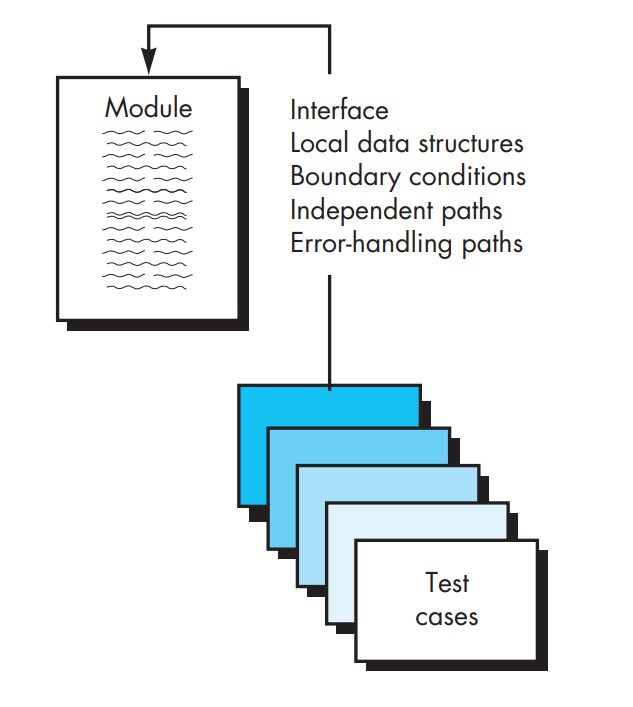
\includegraphics[scale=.4]{img/m3_24}
	\caption{Unit test}
\end{figure}
\end{frame}
\begin{frame}{INTEGRATION TESTING}
\textbf{INTEGRATION TESTING}
\begin{itemize}
	\item Integration testing (sometimes called integration and testing, abbreviated I\&T) is the phase in software testing in which\textbf{ individual software modules are combined and tested as a group. }
	\item Integration testing is conducted to\textbf{ evaluate }the compliance of a \textbf{system or component with specified functional requirements.}
	\item The 
	objective is to \textbf{take unit-tested components and build a program structure }that has been 
	dictated by design
	\item Conducting tests to uncover errors associated with interfacing. 
	
\end{itemize}
\end{frame}

\begin{frame}{INTEGRATION TESTING}
	\textbf{INTEGRATION TESTING Vont...}
	\begin{itemize}
		\item \textbf{Incremental integration} is the antithesis of the big bang approach. 
		\item The \textbf{program is constructed and tested in small increments, }
		\begin{itemize}
			\item where errors are easier to isolate and correct; 
			\item interfaces are more likely to be tested completely; 
			\item and a systematic test approach may be applied. 
		\end{itemize}
		\item A number of different incremental integration strategies are discussed below.
		\begin{enumerate}
			\item Top-Down Integration
			\item Bottom-Up Integration
			\item Regression Testing
			\item Smoke Testing
			
		\end{enumerate}
	\end{itemize}
\end{frame}

\begin{frame}{INTEGRATION TESTING}
\begin{itemize}
	\item[1] Top-Down Integration: 
	\begin{itemize}
		\item \textbf{An incremental approach} to construction of the software architecture. 
		\item \textbf{Modules are integrated by moving downward} through the control hierarchy, \textbf{beginning with the main control module} (main program). 
		\item Modules subordinate to the main control module are \textbf{incorporated }into the structure in either a \textbf{depth-first or breadth-first manner.}
		
	\end{itemize}
\item[2] Bottom-Up Integration
\begin{itemize}
	\item \textbf{Begins} construction and testing with \textbf{atomic modules} (i.e., components at the lowest levels in the program structure). 
	\item Because \textbf{components are integrated from the bottom up}, the \textbf{functionality} provided by components subordinate to a given level is\textbf{ always available} and the need for stubs is eliminated.
	
\end{itemize}
\end{itemize}
\end{frame}
\begin{frame}{INTEGRATION TESTING}
	\begin{itemize}
		\item[3] Regression Testing
		\begin{itemize}
			\item Each time a new module is added as part of integration testing, the software changes. 
			\item New data flow paths are established, new I/O may occur, and new control logic is invoked. 
			\item Side effects associated with these changes may cause problems with functions that previously worked flawlessly. 
			\item In the context of an integration test strategy,\textbf{ regression testing is the re-execution of some subset of tests that have already been conducted to ensure that changes have not propagated unintended side effects. }
			\item Regression testing helps to ensure that changes (due to testing or for other reasons) do not introduce unintended behavior or additional errors.
		\end{itemize}
	\end{itemize}
\end{frame}
\begin{frame}{INTEGRATION TESTING}
	\begin{itemize}
		\item[4] Smoke Testing
		\begin{itemize}
			\item Smoke testing is a type of software testing which\textbf{ ensures that the major functionalities of the application are working fine. }
			\item It is a non-exhaustive testing with very \textbf{limited test cases} to \textbf{ensure that the important features are working fine and we are good to proceed with the detailed testing.}
			\item Smoke testing is an integration testing approach that is commonly used when product software is developed. 
			\item It is designed as a pacing mechanism for time-critical projects, allowing the software team to assess the project on a frequent basis. 
			
		\end{itemize}
	\end{itemize}
\end{frame}

\begin{frame}{VALIDATION TESTING}
	\textbf{VALIDATION TESTING}
	\begin{itemize}
		\item The process of evaluating software during the development process or at the end of the development process \textbf{to determine whether it satisfies specified business requirements.}
		\item Validation Testing\textbf{ ensures that the product actually meets the client's needs.} It can also be defined as to demonstrate that the product fulfills its intended use when deployed on appropriate environment.
		\item \textbf{Quality control comes under validation testing.}
		\item Testing\textbf{ focuses on user-visible actions and user-recognizable output }from the system.
		\item Validation can be defined in many ways, but a simple definition is that validation succeeds when software functions in a manner that can be reasonably expected by the customer. 
		
	\end{itemize}
\end{frame}

\begin{frame}{SYSTEM TESTING}
	\textbf{SYSTEM TESTING}
	\begin{itemize}
		\item System Testing is a type of software testing that is performed on a\textbf{ complete integrated system to evaluate the compliance of the system with the corresponding requirements. }
		\item System Testing is\textbf{ carried out} on the whole system in the context of\textbf{ either system requirement specifications or functional requirement specifications or in the context of both. }
		\item System testing\textbf{ tests }the \textbf{design and behavior of the system }and also \textbf{the expectations of the customer.} 
	\end{itemize}
\end{frame}
\begin{frame}{SYSTEM TESTING}
	\textbf{System Testing Process:}
	\begin{itemize}
		\item Test Environment Setup
		\item Create Test Case
		\item Create Test Data
		\item Execute Test Case
		\item Defect Reporting
		\item Regression Testing
		\item Log Defects
		\item Retest: If the test is not successful then again test is performed.
	\end{itemize}
\end{frame}
\begin{frame}{SYSTEM TESTING}
	\textbf{Types of System Testing:}
	\begin{itemize}
		\item \textbf{Performance Testing:} Performance Testing is a type of software testing that is carried out to test the speed, scalability, stability and reliability of the software product or application.
		\item \textbf{Load Testing:} Load Testing is a type of software Testing which is carried out to determine the behavior of a system or software product under extreme load.
		\item \textbf{Stress Testing:} Stress Testing is a type of software testing performed to check the robustness of the system under the varying loads.
		\item \textbf{Scalability Testing:} Scalability Testing is a type of software testing which is carried out to check the performance of a software application or system in terms of its capability to scale up or scale down the number of user request load.
	\end{itemize}
\end{frame}

\begin{frame}{DEBUGGING}
	\textbf{DEBUGGING}
	\begin{itemize}
		\item Debugging occurs as a consequence of successful testing. That is, when a test case 
		uncovers an error, debugging is the process that results in the removal of the error.
		\item The debugging process will usually have one of two outcomes:
		\begin{itemize}
			\item The cause will be found and 
			corrected or
			\item The cause will not be found
		\end{itemize}
	\end{itemize}
\end{frame}
\begin{frame}{DEBUGGING}
\begin{figure}
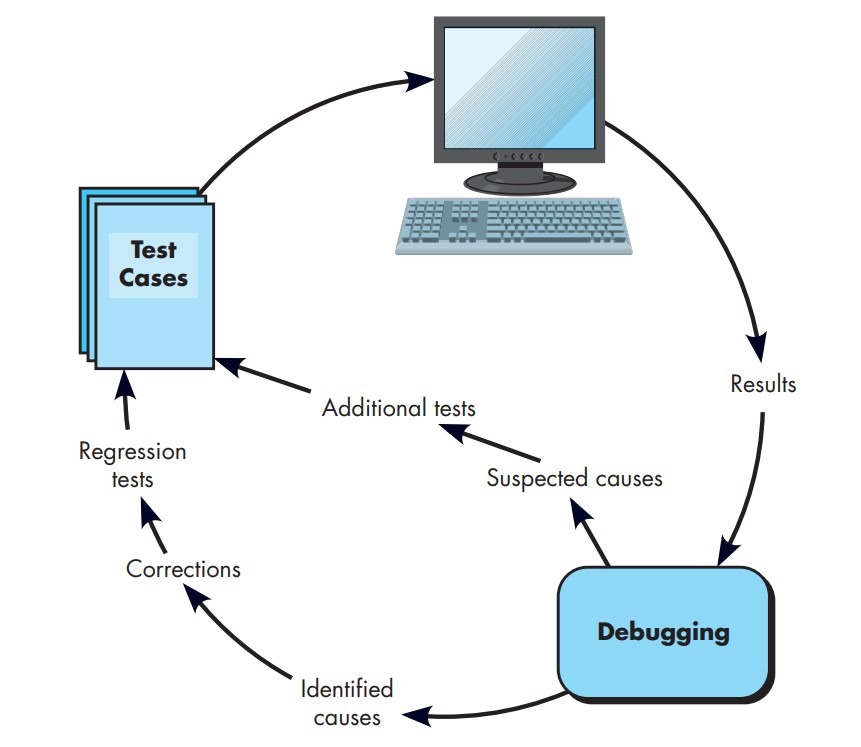
\includegraphics[scale=.4]{img/m3_25}
\caption{The 
	debugging 
	process}
\end{figure}
\end{frame}
\begin{frame}{DEBUGGING}
	\textbf{Strategies:}
\begin{itemize}
	\item \textbf{The brute force:} It is the most common method of debugging but is the least efficient method. In this approach, print statements are inserted throughout the program to print the intermediate values with the hope that some of the printed values will help to identify the statement in error. 
	\item \textbf{Backtracking:}This is also a fairly common approach. In this approach, starting from the statement at which an error symptom has been observed, the source code is traced backwards until the error is discovered. Unfortunately, as the number of source lines to be traced back increases, the number of potential backward paths increases.
	\item \textbf{Cause elimination method:}In this approach, once a failure is observed, the symptoms of the failure are noted. Based on the failure symptoms, the causes which could have contributed to the symptom are developed and tests are conducted to eliminate each. A related technique of identification of the error from the error symptom is the software fault tree analysis.
\end{itemize}
\end{frame}
\begin{frame}{White box testing}
\textbf{White box testing}
\begin{itemize}
	\item White-box testing (also known as clear box testing, glass box testing, transparent box testing, and structural testing) is a method of software testing that \textbf{tests internal structures or working of an application.}
	\item White-box testing can be applied at the unit, integration and system levels of the software testing process.
\end{itemize}
\end{frame}
\begin{frame}{White box testing}
	\textbf{White box testing cont..}
	\begin{itemize}
		\item Using white-box testing methods, you can derive test cases that 
		\begin{itemize}
			\item guarantee that all independent paths within a module have been exercised at least once, 
			\item exercise all logical decisions on their true and false sides, 
			\item execute all loops at their boundaries and within their operational bounds, and 
			\item exercise internal data structures to ensure their validity.
			
		\end{itemize}
	\item It is mostly done by software developers
	\item Knowledge of implementation is required.
	\item It is the inner or the internal software testing.
	
	\end{itemize}
\end{frame}
\begin{frame}{Path testing}
	\textbf{Path testing}
	\begin{itemize}
		\item Basis Path Testing in software engineering is a White Box Testing method in which test cases are defined based on flows or logical paths that can be taken through the program. 
		\item The objective of basis path testing is to\textbf{ define the number of independent paths, so the number of test cases needed can be defined explicitly to maximize test coverage.}
		\item Test cases derived to exercise the basis set are guaranteed to execute every statement in the program at least one time during testing.
	\end{itemize}
\end{frame}
\begin{frame}{Path testing}
	\textbf{Path Testing Process:}
	\begin{itemize}
		\item Draw the corresponding control flow graph of the program in which all the executable paths are to be discovered.(Control Flow Graph)
		\item After the generation of the control flow graph, calculate the cyclomatic 
		complexity of the program using the following formula.(Cyclomatic Complexity)
		\begin{itemize}
			\item McCabe's $Cyclomatic \  Complexity\  = E - N + 2P$\\
			Where, E = Number of edges in control flow graph\\ N = Number of vertices in control flow graph\\ P =
			Program factor
		\end{itemize}
	\item Make a set of all the path according to the control flow graph and calculated. The cardinality 
	of set is equal to the calculated cyclomatic complexity.
(Make Set)
	\item Create Test Cases: Create test case for each path of the set obtained in above step.
	\end{itemize}
\end{frame}
\begin{frame}{Path testing}
	\textbf{Path Testing Techniques:}
	\begin{itemize}
		\item \textbf{Control Flow Graph:} The program is converted into control flow graph by representing the code into 
		nodes and edges.
		\item \textbf{Decision to Decision path:} The control flow graph can be broken into various Decision to Decision paths 
		and then collapsed into individual nodes.
		\item \textbf{Independent paths:} Independent path is a path through a Decision-to-Decision path graph which 
		cannot be reproduced from other paths by other methods.
		
	\end{itemize}
\end{frame}
\begin{frame}{Control Structure testing}
	\textbf{Control Structure testing}
	\begin{itemize}
		\item Control structure testing is a group of white-box testing methods.
		\item Control structure testing is used to increase the coverage area by testing various control structures present in the program. \item The different types of testing performed under control structure testing are as follows
		\begin{enumerate}
			\item Condition Testing 
			\begin{itemize}
				\item Condition testing is a test cased design method, which ensures that the logical condition and decision statements are free from errors.
			\end{itemize}
			\item Data Flow Testing
			\begin{itemize}
				\item he data flow test method chooses the test path of a program based on the locations of the definitions and uses all the variables in the program. 
			\end{itemize}
			\item Loop Testing 
			\begin{itemize}
				\item Loop testing is actually a white box testing technique. It specifically focuses on the validity of loop construction.
			\end{itemize}
		\end{enumerate}
		
	\end{itemize}
\end{frame}
\begin{frame}{Control Structure testing}
There are four different classes of loops
\begin{itemize}
	\item Simple Loop
	\item Nested Loop
	\item Concatenated Loop
	\item Unstructured Loop
\end{itemize}
\end{frame}
\begin{frame}{Control Structure testing}
\textbf{Simple Loop Testing}
	\begin{itemize}
		\item A simple loop is tested in the following way:
		\begin{enumerate}
			\item Skip the entire loop.
			\item Make 1 pass through the loop.
			\item Make 2 passes through the loop.
			\item Make m passes through the loop where $m<n$, n is the maximum number of passes through the loop.
			\item Make $n, n-1, n+1 $ passes through the loop.
		\end{enumerate}
	\end{itemize}
\textbf{Nested Loop Testing}
\begin{itemize}
	\item A nested loop is tested in the following way.
	\begin{enumerate}
		\item Start the innermost loop.
		\item Conduct a simple loop test for the innermost loop.
		\item Work outward, conducting a test for the next loop keeping all other loops at a minimum.
		\item Continue until all the loops are tested.
	\end{enumerate}
\end{itemize}
\end{frame}
\begin{frame}{Control Structure testing}
\textbf{Concatenated Loop Testing}
\begin{itemize}
	\item To test the concatenated loops, the procedure is
	\begin{enumerate}
		\item if the loops are independent then test them as simple loops \item otherwise test them as nested loops.
	\end{enumerate}
\end{itemize}
\textbf{Unstructured Loop Testing}
\begin{itemize}
	\item To test the unstructured loops we needs to restructure their design.
\end{itemize}
\end{frame}
\begin{frame}{Control Structure testing}
	\begin{figure}
		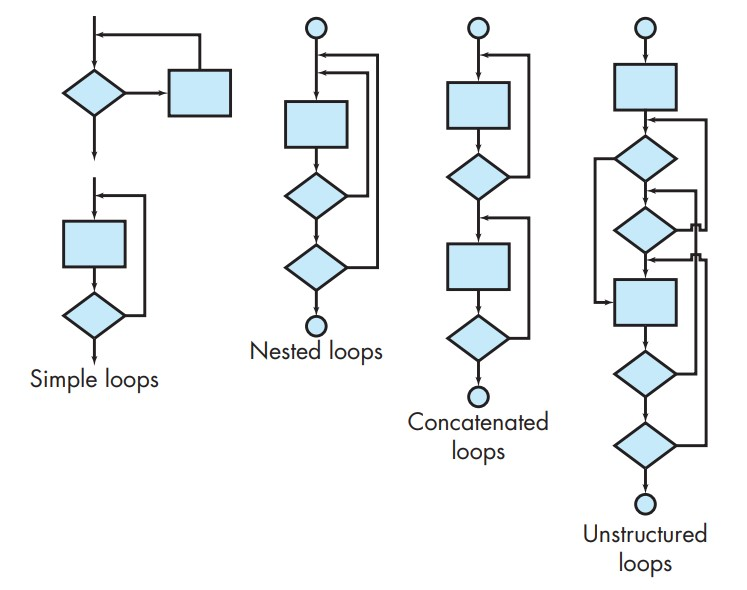
\includegraphics[scale=.4]{img/m3_26}
		\caption{Classes of Loops}
	\end{figure}
\end{frame}
\begin{frame}{Black box testing}
\textbf{Black box testing}
\begin{itemize}
	\item Black Box Testing is a software testing method in which the functionalities of software applications are\textbf{ tested without having knowledge of internal code structure, implementation details and internal paths. }
\begin{itemize}
	\item That is, black-box testing techniques enable you to derive sets of input conditions that will fully exercise all functional requirements for a program. 
\end{itemize}
	\item That is, black-box testing techniques enable you to derive sets of input conditions that will fully exercise all functional requirements for a program. 
	\item Black-box testing attempts to find errors in the following categories: 
	\begin{itemize}
		\item incorrect or missing functions, 
		\item interface errors, 
		\item errors in data structures or external database access, 
		\item behavior or performance errors, and 
		\item initialization and termination errors.
	\end{itemize}
\item Blackbox testing tends to be applied during later stages of testing.
\end{itemize}
\end{frame}
\begin{frame}{Test documentation}
	\textbf{Test documentation}
\begin{itemize}
	\item Test documentation is documentation of artifacts created before or during the testing of software.
	\item It helps the testing team to estimate testing effort needed, test coverage, resource tracking, execution progress, etc. 
	\item The main reason behind creating test documentation is to either reduce or remove any uncertainties 
	about the testing activities.
	\item Helps you to remove ambiguity which often arises when it comes to the 
	allocation of tasks
	\item Documentation not only offers a systematic approach to software testing, but it also acts as training 
	material to freshers in the software testing process
	\item Test documentation helps you to offer a quality product to the client within specific time limits.

\end{itemize}
\end{frame}
\begin{frame}{Test documentation}
	\begin{figure}
	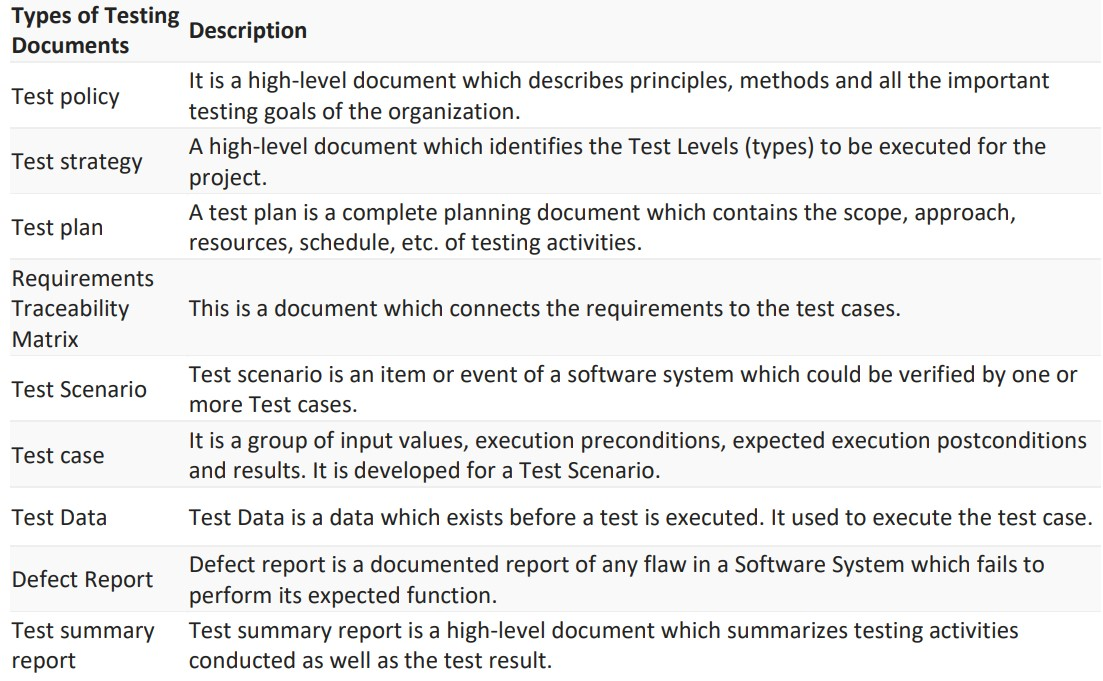
\includegraphics[scale=.5]{img/m3_51}
	%	\caption{Classes of Loops}
\end{figure}
\end{frame}
\begin{frame}{Test documentation}
	\begin{figure}
	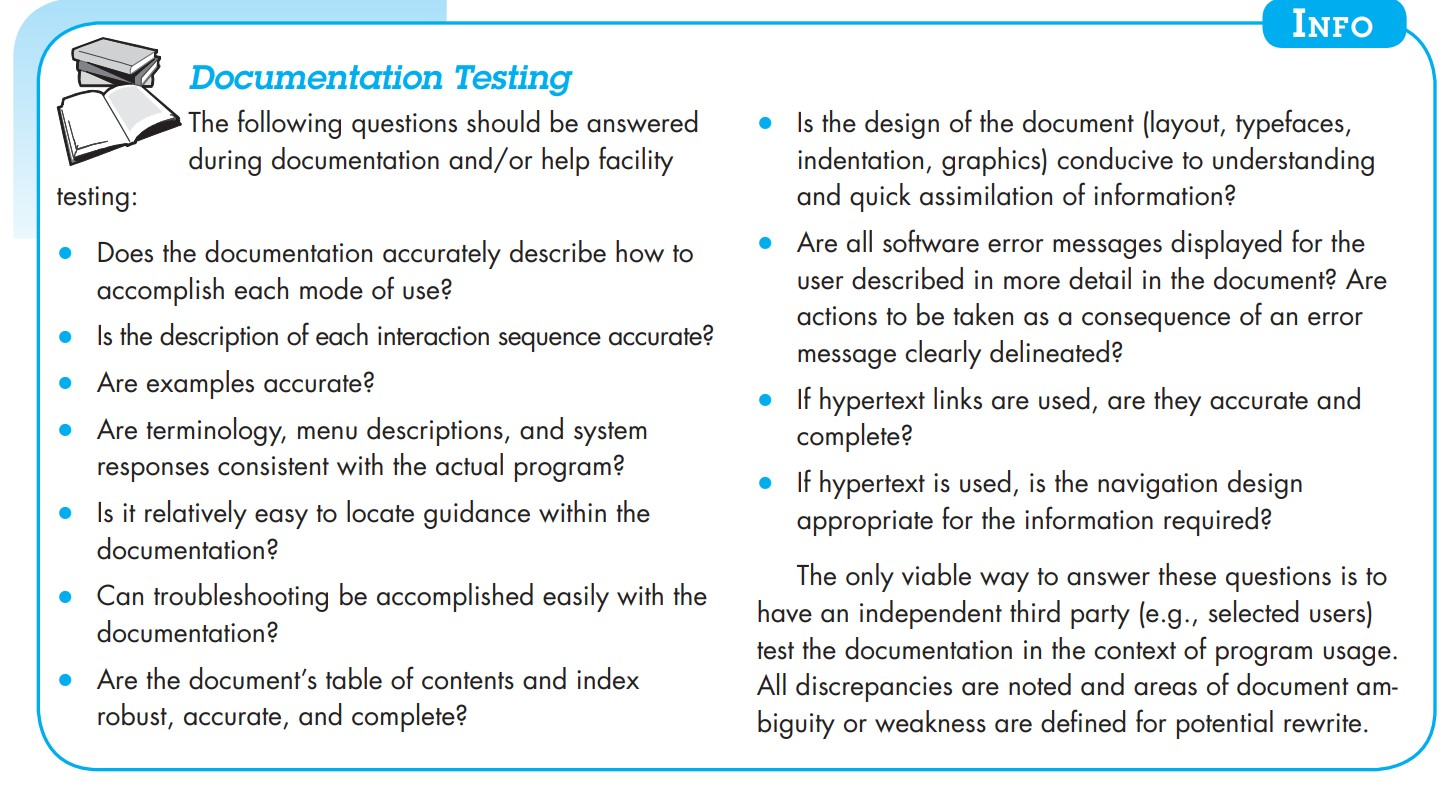
\includegraphics[scale=.4]{img/m3_27}
%	\caption{Classes of Loops}
\end{figure}
\end{frame}
\begin{frame}{Test automation}
	\textbf{Test automation}
	\begin{itemize}
		\item Automated testing is based on the idea that tests should be executable. 
		\item An executable test includes the input data to the unit that is being tested, the expected result and a check that the unit returns the expected result. 
		\item Can run the test and the test passes if the unit returns the expected result. 
		\item Normally, hundreds or thousands of executable tests are developed for a software product.
		
	\end{itemize}
\end{frame}
\begin{frame}{Test automation}
	\begin{figure}
	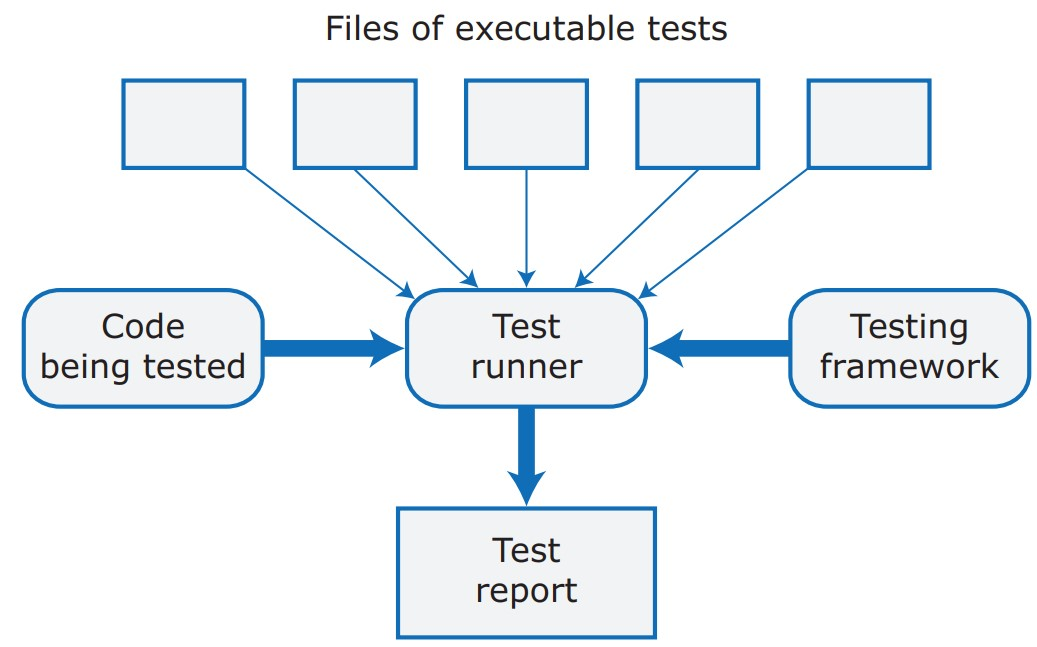
\includegraphics[scale=.4]{img/m3_28}
		\caption{Automated testing}
\end{figure}
\end{frame}
\begin{frame}{Test automation}
\textbf{Automated tests}
\begin{itemize}
	\item It is good practice to structure automated tests into three parts:
	\begin{itemize}
		\item \textbf{Arrange} can set up the system to run the test. This involves defining the test parameters and, if necessary, mock objects that emulate the functionality of code that has not yet been developed.
	\item \textbf{Action} can call the unit that is being tested with the test parameters. 
		\item \textbf{Assert} can make an assertion about what should hold if the unit being tested has executed successfully.For example AssertEquals, which checks if its parameters are equal.
	\end{itemize}
\item Can use equivalence partitions to identify test inputs, should have several automated tests based on correct and incorrect inputs from each partition. 

\end{itemize}
\end{frame}
\begin{frame}{Automated tests}
\textbf{Testing Pyramid}
\begin{itemize}
	\item Mike Cohn  proposed the testing pyramid, suggests that $70\%$ of automated tests should be unit tests, $20\%$ feature tests(called these service tests), and $10\%$ system tests (UI tests).
	\item The implementation of system features usually involves integrating functional units into components and then integrating these components to implement the feature.
	\item If you have good unit tests, then be confident that the individual functional units and components that implement the feature will behave as expected. 
\end{itemize}
\end{frame}
\begin{frame}{Test automation}
	\begin{figure}
		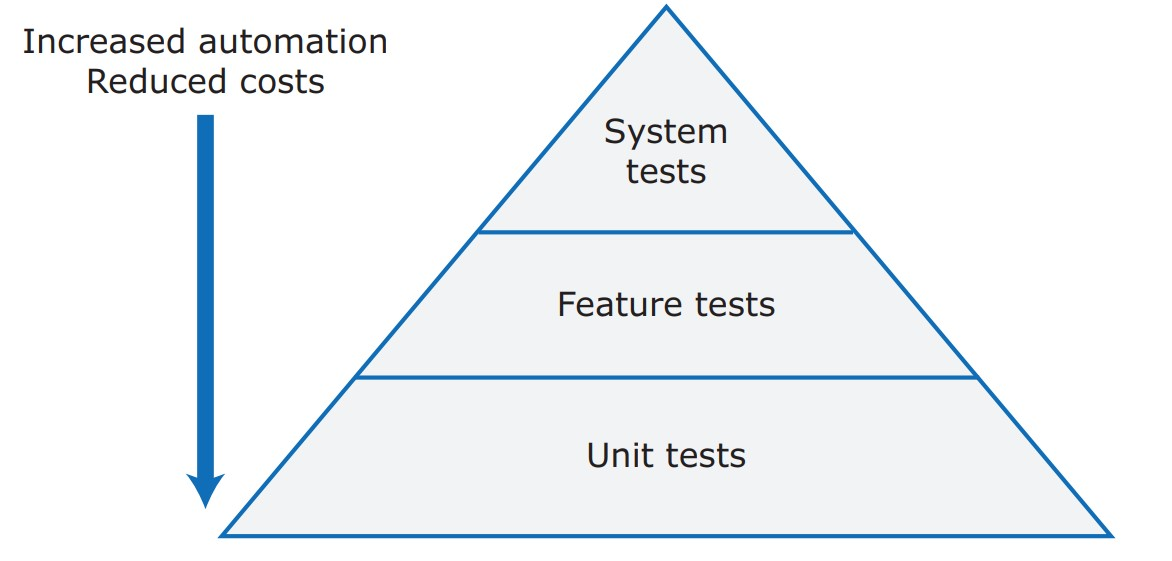
\includegraphics[scale=.4]{img/m3_29}
		\caption{The test pyramid}
	\end{figure}
\end{frame}
\begin{frame}{Test automation}
	\textbf{Automated feature testing}
	\begin{itemize}
		\item \textbf{Generally, users access features through the product’s graphical user interface (GUI)}. 
		\item \textbf{GUI-based testing is expensive to automate} so it is best to design your product \textbf{so that its features can be directly accessed through an API }and not just from the user interface. 
		\item The feature tests can then access features directly through the API without the need for direct user interaction through the system’s GUI. 
		\item Accessing features through an API has the additional benefit that it is possible to re-implement the GUI without changing the functional components of the software.
		
	\end{itemize}
\end{frame}
\begin{frame}{Test automation}
	\begin{figure}
		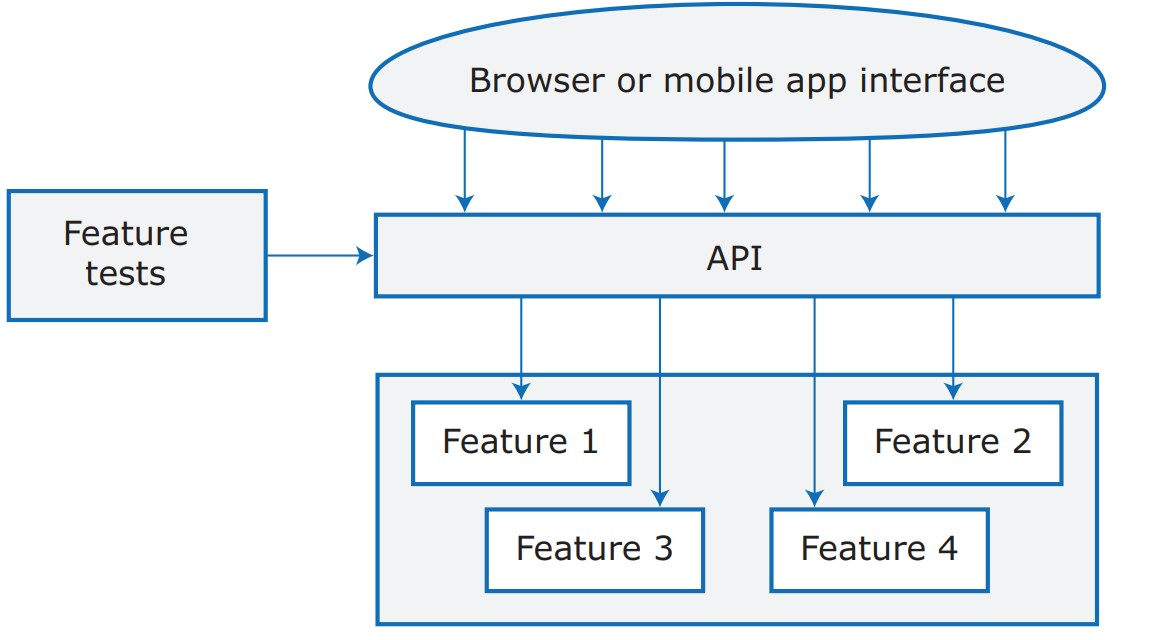
\includegraphics[scale=.4]{img/m3_30}
		\caption{Feature testing through an API}
	\end{figure}
\end{frame}

\begin{frame}{Test-driven development}
	\textbf{Test-driven development}
	\begin{itemize}
		\item Test-driven development (TDD) is an approach to program development that is based around the general idea that you should w\textbf{rite an executable test or tests for code} that you are writing \textbf{before you write the code}. 
		\item It was introduced by early users of the Extreme Programming agile method, but it can be used with any incremental development approach.
		\item \textbf{Test-driven development works best for the development of individual program units} and \textbf{it is more difficult to apply to system testing}. 
		\item Even the strongest advocates of TDD accept that it is challenging to use this approach when you are developing and testing systems with graphical user interfaces.
	\end{itemize}
\end{frame}
\begin{frame}{Test-driven development}
	\begin{figure}
		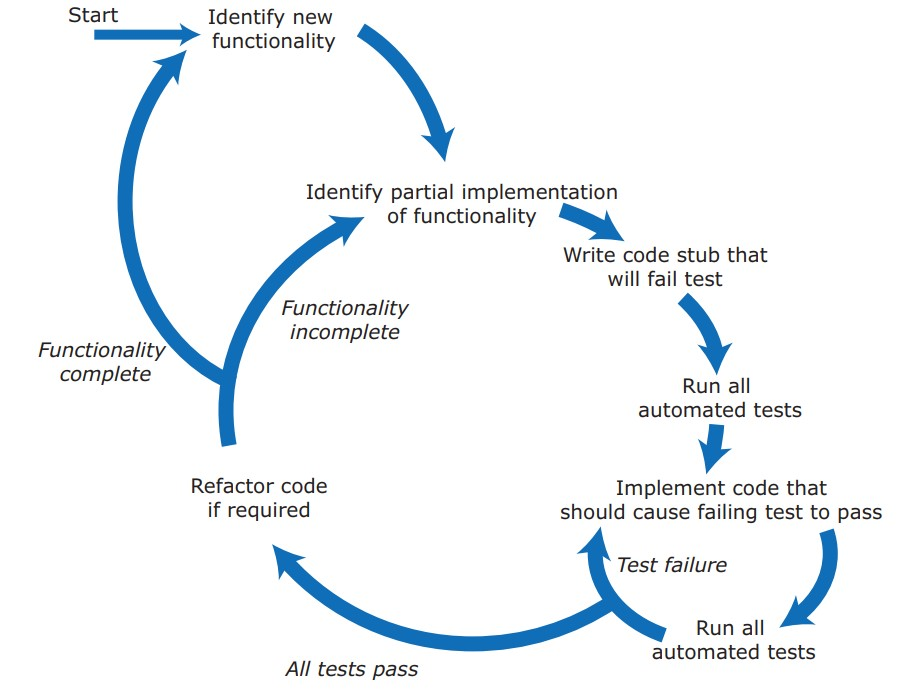
\includegraphics[scale=.4]{img/m3_31}
		\caption{Test-driven development}
	\end{figure}
\end{frame}
\begin{frame}{Test-driven development}
	\begin{itemize}
		\item Assume that we have identified some increment of functionality to be implemented. 
		\item Test-driven development relies on automated testing. Every time you add some functionality, you develop a new test and add it to the test suite. 
		\item All of the tests in the test suite must pass before you move on to developing the next increment.
		
	\end{itemize}
\end{frame}
\begin{frame}{Test-driven development}
	\begin{figure}
		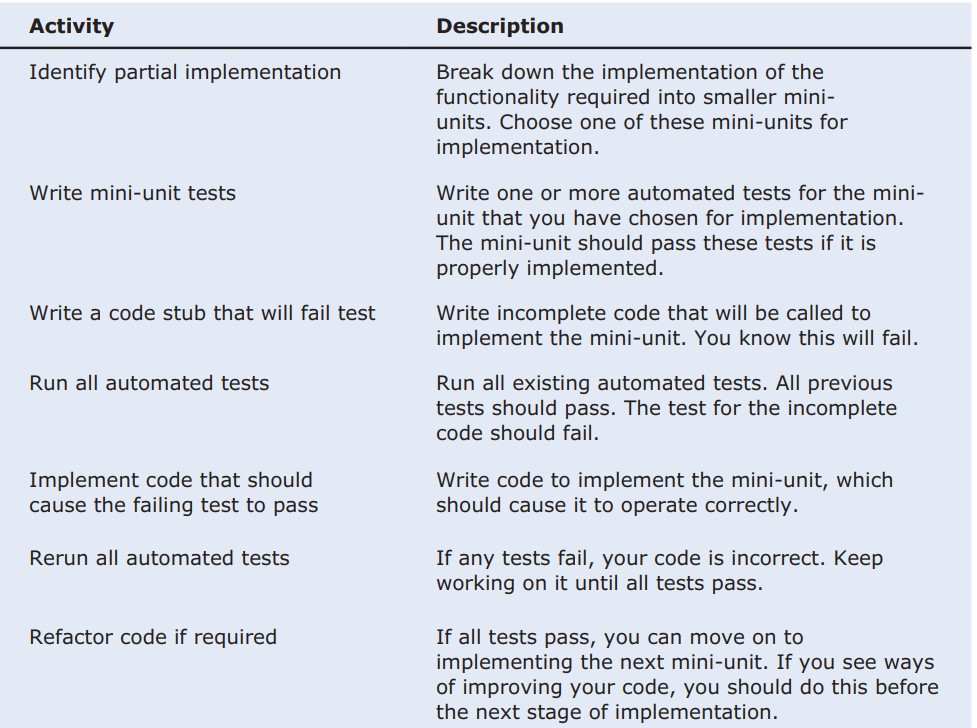
\includegraphics[scale=.45]{img/m3_32}
		\caption{Stages of test-driven development}
	\end{figure}
\end{frame}
\begin{frame}{Test-driven development}
	\textbf{Benefits of test-driven development}
	\begin{itemize}
		\item It is a systematic approach to testing in which tests are clearly linked to sections of the program code. 
		\begin{itemize}
			\item This means it is been confident that the tests cover all of the code that has been developed and that there are no untested code sections in the delivered code.This is the most significant benefit of TDD. 
		\end{itemize}
	\item The tests act as a written specification for the program code. In principle at least, it should be possible to understand what the program does by reading the tests. 
	\item Debugging is simplified because, when a program failure is observed, it can immediately link this to the last increment of code that have  added to the system.
	\item It is argued that TDD leads to simpler code as programmers only write code that’s necessary to pass tests. They don’t over-engineer their code with complex features that aren’t needed.
	
	\end{itemize}
\end{frame}

\begin{frame}{Security testing}
	\textbf{Security testing}
	\begin{itemize}
		\item Security testing aims to \textbf{find vulnerabilities} that may be exploited by an attacker and to \textbf{provide convincing evidence that the system is sufficiently secure.} 
		\item The tests should demonstrate that the system can resist attacks on its availability, attacks that try to inject malware and attacks that try to corrupt or steal users’ data and identity.
		\item Comprehensive security testing requires specialist knowledge of software vulnerabilities and approaches to testing that can find these vulnerabilities. 
		
	\end{itemize}
\end{frame}
\begin{frame}{Security testing}
	\textbf{Risk-based security testing}
	\begin{itemize}
		\item A risk-based approach to security testing involves \textbf{identifying common risks and developing tests to demonstrate that the system protects itself from these risks}. 
		\item Can also \textbf{use automated tools} that scan the system to \textbf{check for known vulnerabilities}, such as unused HTTP ports being left open.
		\item Based on the risks that have been identified, then design tests and checks to see if the system is vulnerable. 
		\item It may be possible to construct automated tests for some of these checks, but others inevitably involve manual checking of the system’s behaviour and its files.
	\end{itemize}
\end{frame}
\begin{frame}{Security testing}
	\textbf{Examples of security risks}
	\begin{itemize}
		\item Unauthorized attacker gains access to a system using authorized credentials
		\item Authorized individual accesses resources that are forbidden to them
		\item Authentication system fails to detect unauthorized attacker
		\item Attacker gains access to database using SQL poisoning attack
		\item Improper management of HTTP session
		\item HTTP session cookies revealed to attacker
		\item Confidential data are unencrypted
		\item Encryption keys are leaked to potential attackers
		
	\end{itemize}
\end{frame}
\section{DevOps and Code Management}


\begin{frame}{DevOps and Code Management}
	\textbf{DevOps}
	\begin{itemize}
		\item \textbf{To speed up the release and support processes}, an alternative approach called DevOps has been developed.
		\item \textbf{DevOps} (development + operations) \textbf{integrates development, deployment, and support, with a single team responsible for all of these activities}.
		\item Three factors led to the development and widespread adoption of DevOps:
		\begin{itemize}
			\item \textbf{Agile} software engineering reduced the development time for software, but the traditional release process introduced a bottleneck between development and deployment.  
			\item \textbf{Amazon} re-engineered their software around services and introduced an approach in which a service was developed and supported by the same team. Amazon’s claim that this led to significant improvements in reliability was widely publicized.
			\item It became possible to release software as a service, running on a\textbf{ public or private cloud}. Software products did not have to be released to users on physical media or downloads.		
		\end{itemize}
	\end{itemize}
\end{frame}
\begin{frame}{DevOps and Code Management}
	\begin{figure}
	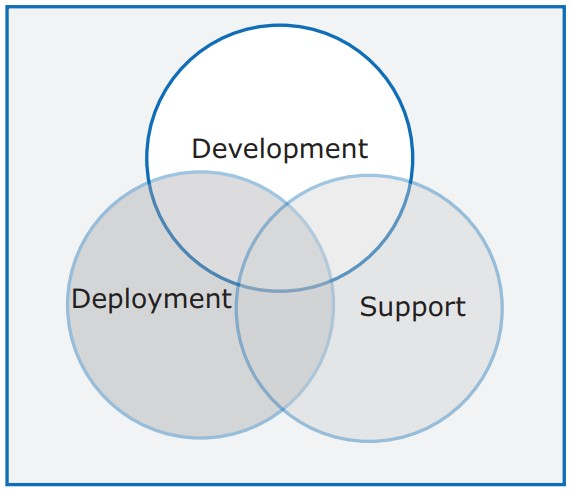
\includegraphics[scale=.45]{img/m3_35}
	\caption{Multi-skilled DevOps team}
\end{figure}
\end{frame}
\begin{frame}{DevOps and Code Management}
	\textbf{DevOps principles}
	\begin{itemize}
		\item Everyone is responsible for 
		everything.
		\item Everything that can be automated 
		should be automated.
		\item Measure first, change later.
		\begin{itemize}
			\item DevOps should be driven by a measurement program where you collect data about the system and its operation. Then use the collected data to inform decisions about changing DevOps processes and tools.
			
		\end{itemize}
	\end{itemize}
\end{frame}
\begin{frame}{DevOps and Code Management}
\textbf{Benefits of DevOps}
\begin{itemize}
	\item Faster deployment
	\item Reduced risk
	\item Faster repair
	\item More productive teams
\end{itemize}
\end{frame}
\begin{frame}{Code Management}
	\begin{figure}
		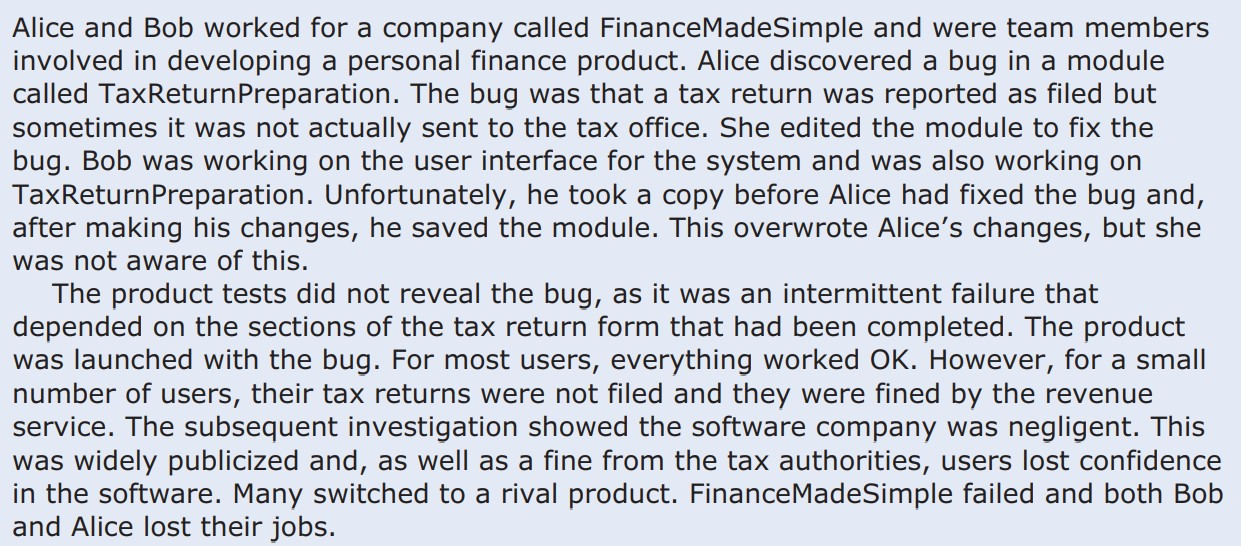
\includegraphics[scale=.45]{img/m3_36}
		\caption{A code management problem}
	\end{figure}
\end{frame}
\begin{frame}{Code Management}
\textbf{Code management}
\begin{itemize}
	\item Code management is a \textbf{set of software-supported practices that is used to manage an evolving codebase}. 
	\item Code management need to \textbf{ensure that}
	\begin{itemize}
		\item  \textbf{changes made} by\textbf{ different developers do not interfere} with each other and to create different product versions. 
	\end{itemize} 
	\item Code management tools make it easy to create an executable product from its source code files and to run automated tests on that product.
\end{itemize}
\end{frame}

\begin{frame}{Code Management}
	\textbf{Code management and DevOps }
	\begin{itemize}
		\item Source code management, combined with automated system building, is essential for professional software engineering. 
		\item In companies that use DevOps, a modern code management system is a fundamental requirement for ‘automating everything’. 
		\item Not only does it store the project code that is ultimately deployed, it also stores all other information that is used in DevOps processes. 
		\item DevOps automation and measurement tools all interact with the code management system
	\end{itemize}
\end{frame}
\begin{frame}{DevOps and Code Management}
	\begin{figure}
		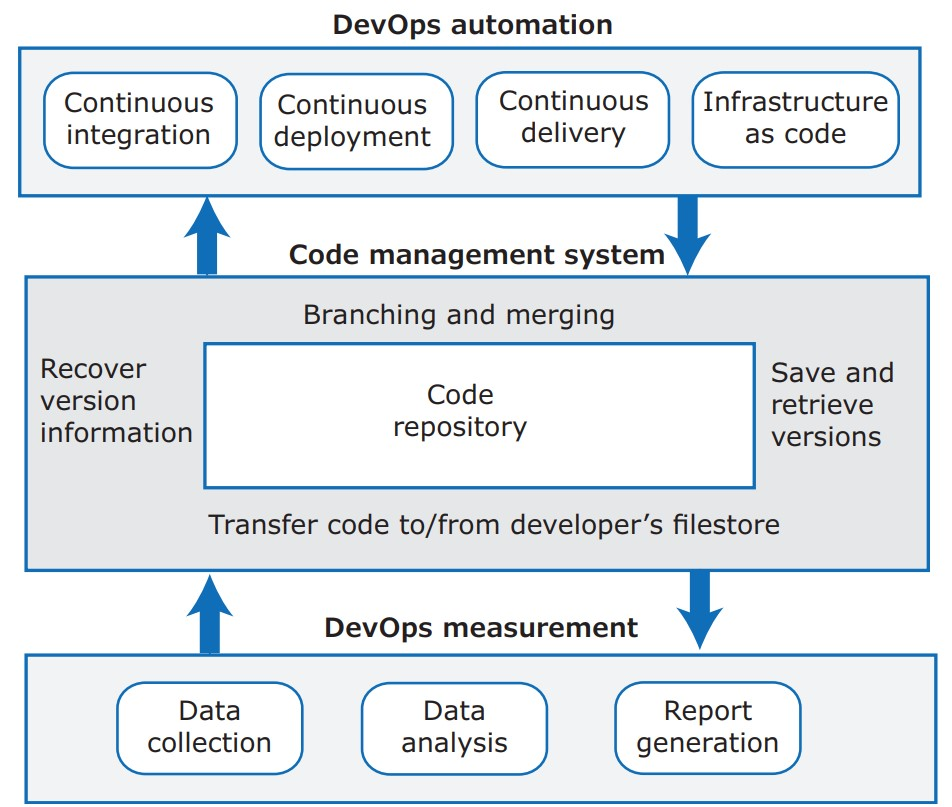
\includegraphics[scale=.4]{img/m3_38}
		\caption{Code management and DevOps}
	\end{figure}
\end{frame}
\begin{frame}{Code Management}
	\textbf{Fundamentals of source code management}
	\begin{itemize}
		\item Code management systems provide a set of features that support four general areas:
		\begin{itemize}
			\item \textbf{Code transfer} Developers take code into their personal file store to work on it then return it to the shared code management system.
			\item \textbf{Version storage and retrieval} Files may be stored in several different versions and specific versions of these files can be retrieved.
			\item \textbf{Merging and branching} Parallel development branches may be created for concurrent working. Changes made by developers in different branches may be merged.
			\item \textbf{Version information} Information about the different versions maintained in the system may be stored and retrieved
			
		\end{itemize}
	\end{itemize}
\end{frame}
\begin{frame}{Fundamentals of source code management}
	\begin{figure}
	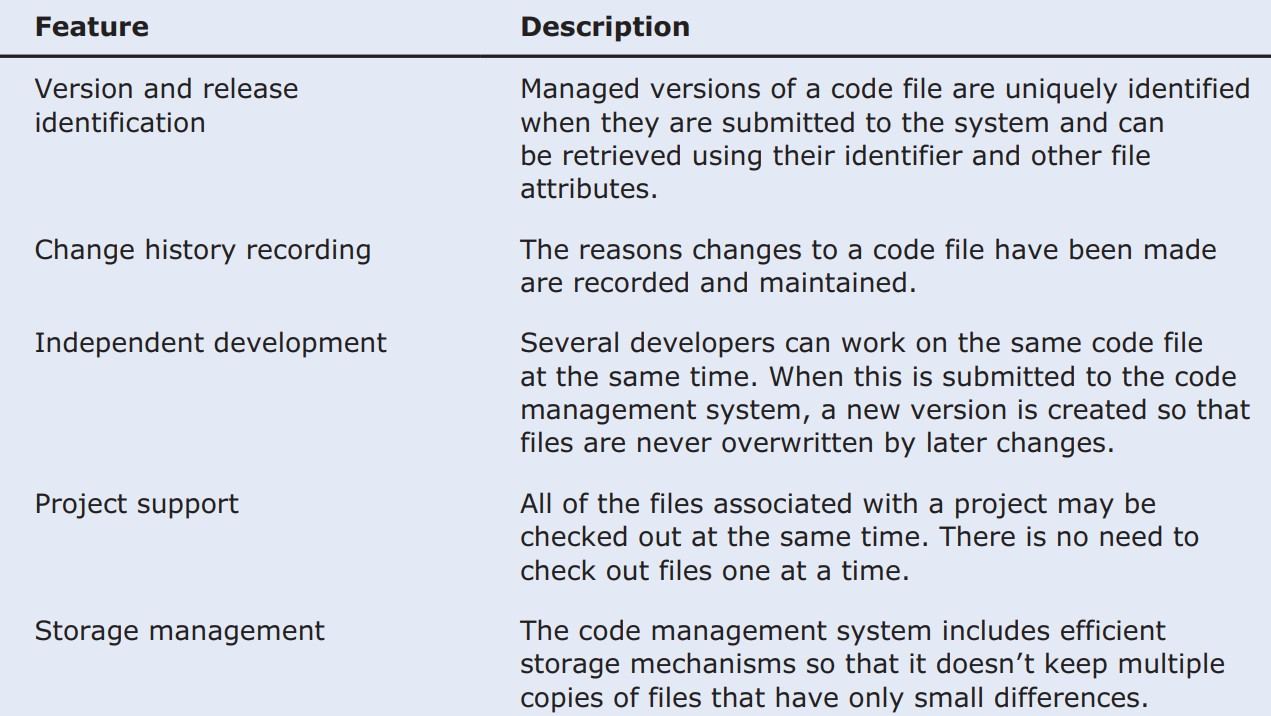
\includegraphics[scale=.4]{img/m3_37}
	\caption{Features of source code management systems}
\end{figure}
\end{frame}
\begin{frame}{Fundamentals of source code management}
	\textbf{Code repository}
	\begin{itemize}
		\item 	All source code management systems have the general form with a shared repository and a set of features to manage the files in that repository:
		
		\begin{itemize}
			\item All source code files and file versions are stored in the repository, as are other artefacts such as configuration files, build scripts, shared libraries and versions of tools used.
			\item Files can be transferred to and from the repository and information about the different versions of files and their relationships may be updated. Specific versions of files and information about these versions can always be retrieved from the repository.
			
		\end{itemize}
	\end{itemize}
\end{frame}

\begin{frame}{Code Management}
	\textbf{Git}
	\begin{itemize}
		\item Git is an \textbf{open-source Version Control System (VCS)}, it is completely free. 
		\item Git is designed to work in small to large level projects.
		\item  Git will help to merge and maintain the history of code changes.
		\item  Github is the repository where all the source code is kept by Git users.
		\item GitHub offers local branching and multiple workflows. 
		\item Instead of only keeping the copies of the files that users are working on, \textbf{Git maintains a clone of the repository on every user’s computer }
		\item A \textbf{fundamental concept in Git} is the \textbf{“master branch,”} which is the current master version of the software that the team is working on.
	\end{itemize}
\end{frame}


\begin{frame}{Code Management}
		\begin{figure}
		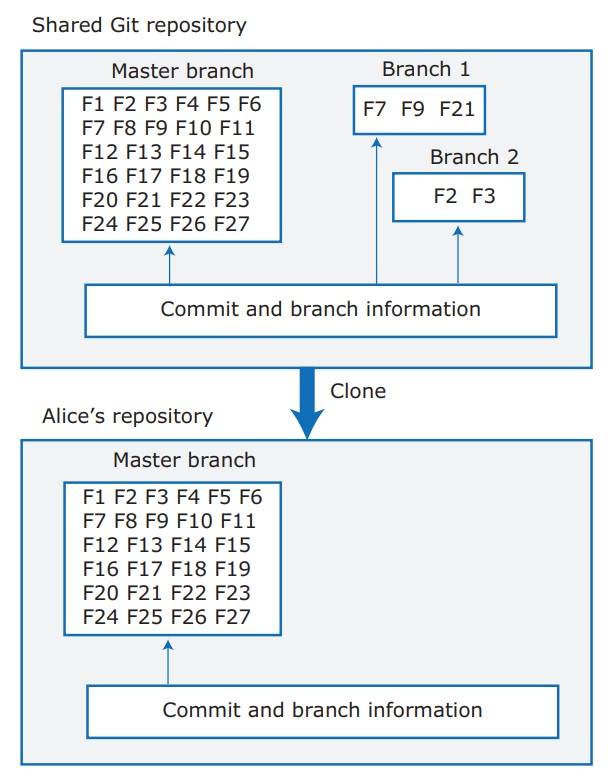
\includegraphics[scale=.4]{img/m3_39}
		\caption{Repository cloning in Git}
	\end{figure}
\end{frame}
\begin{frame}{Code Management}
	\textbf{Benefits of distributed code management}
	\begin{itemize}
		\item Resilience
		\begin{itemize}
			\item \textbf{Everyone working on a project has their own copy} of the repository. \textbf{If the shared repository is damaged }or subjected to a cyberattack, work can continue, and the \textbf{clones can be used to restore the shared repository}. People can work offline if they don’t have a network connection.
		\end{itemize}
		\item Speed
			\begin{itemize}
			\item Committing changes to the repository is a fast, local operation and does not need data to be transferred over the network. 
		\end{itemize}
		\item Flexibility
			\begin{itemize}
			\item \textbf{Local experimentation is much simpler.} Developers can safely experiment and try different approaches without exposing these to other project members. With a centralized system, this may only be possible by working outside the code management system.
		\end{itemize}
		
		
	\end{itemize}
\end{frame}
\begin{frame}{Code Management}
	\begin{figure}
		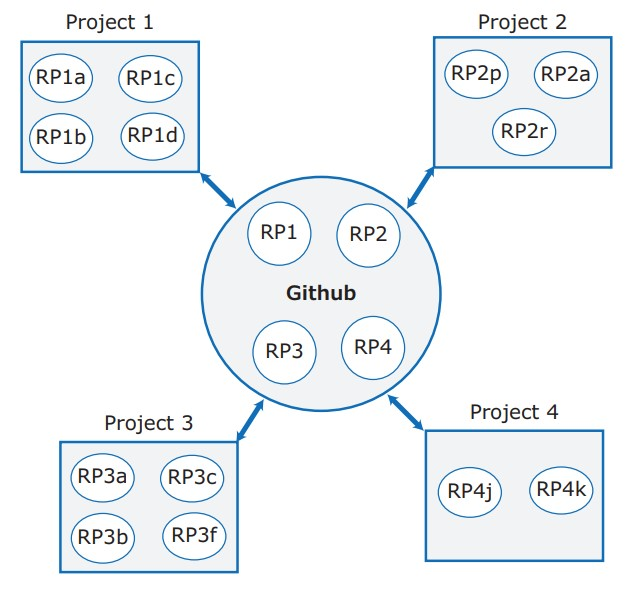
\includegraphics[scale=.4]{img/m3_40}
		\caption{Git repositories}
	\end{figure}
\end{frame}
\begin{frame}{Code Management}
\textbf{Git Cont..}
\begin{itemize}
	\item Most software product companies now use Git for code management.
	\item For teamwork, Git is organized around the notion of a shared project repository and private 
	clones of that repository held on each developer’s computer .
	\item A company may use its own server to run the project repository. However, many 
	companies and individual developers use an external Git repository provider. 
	\item Several Git repository \textbf{hosting companies, such as Github and Gitlab}, host thousands of 
		repositories on the cloud. 
\end{itemize}

\end{frame}
\begin{frame}{Code Management}
	\textbf{Git Cont..}
\begin{itemize}
	\item Figure  shows four project repositories on Github, RP1–RP4. RP1 is the repository for project 1, 
	 RP2 is the repository for project 2, and so on. Each of the developers on each project is identified 
	by a letter (a, b, c, etc.) and has an individual copy of the project repository. 
	\item Developers may work on more than one project at a time, so they may have copies of several Git 
	repositories on their computer.
	\item For example, developer a works on Project 1, Project 2, and Project 3, so has clones of RP1, RP2, 
	and RP3.
\end{itemize}
\end{frame}
\begin{frame}{DevOps automation}
\textbf{DevOps automation}
\begin{itemize}
	\item By using \textbf{DevOps with automated support,} can dramatically \textbf{reduce the time and costs for integration, deployment and delivery.}
	\item Everything that can be, should be automated is a fundamental principle of DevOps. 
	\item As well as reducing the costs and time required for integration, deployment and delivery, process automation also makes these processes more reliable and reproducible. 
	\item Automation information is encoded in scripts and system models that can be checked, reviewed, versioned and stored in the project repository.
\end{itemize}
\end{frame}
\begin{frame}{DevOps automation}
	\begin{figure}
		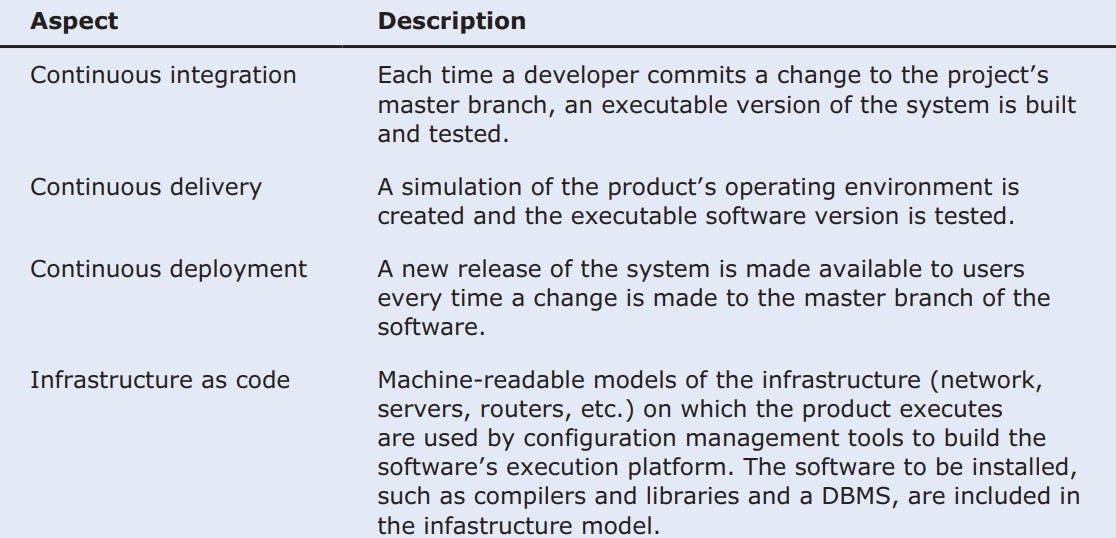
\includegraphics[scale=.5]{img/m3_41}
		\caption{Aspects of DevOps automation}
	\end{figure}
\end{frame}
\begin{frame}{DevOps automation}
	\textbf{Continuous integration}
	\begin{itemize}
		\item Continuous integration simply means that an \textbf{integrated version of the system is created and tested every time a change is pushed to the system’s shared repository. }
		\item On completion of the push operation, the repository sends a message to an integration server to build a new version of the product
		\item The \textbf{advantage of continuous} integration compared to less frequent integration is that it is\textbf{ faster to find and fix bugs in the system. }
		\item If a small change  are made and some system tests then fail, the problem almost certainly lies in the new code that  have pushed to the project repo. 
		\item Focus on this code to find the bug that’s causing the problem. 
		
	\end{itemize}
\end{frame}
\begin{frame}{DevOps automation}
	\begin{figure}
		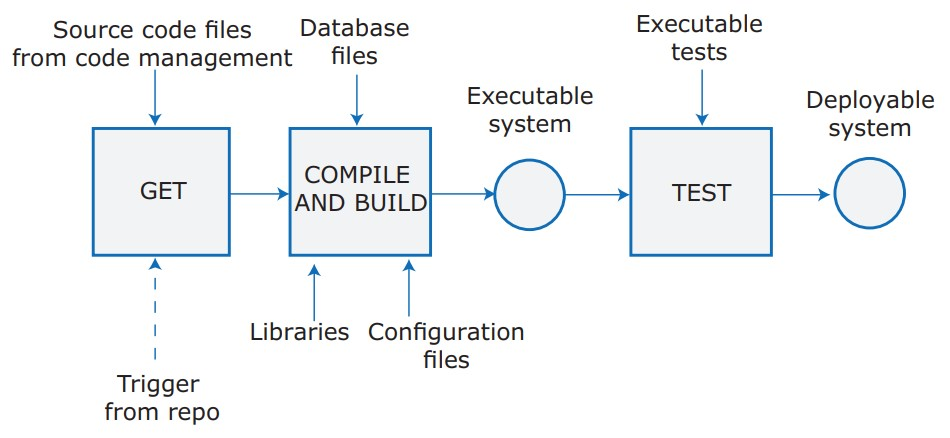
\includegraphics[scale=.5]{img/m3_42}
		\caption{Continuous integration}
	\end{figure}
\end{frame}
\begin{frame}{DevOps automation}
	\textbf{Continuous delivery and deployment}
	\begin{itemize}
		\item Continuous integration means creating an executable version of a software system whenever a change is made to the repository. The CI tool builds the system and runs tests on your development computer or project integration server. 
		\item However, the real environment in which software runs will inevitably be different from your development system. 
		\item When your software runs in its real, operational environment bugs may be revealed that did not show up in the test environment.
		\item \textbf{Continuous delivery means that, after making changes to a system, you ensure that the changed system is ready for delivery to customers.}
		\item This means that you have to test it in a production environment to make sure that environmental factors do not cause system failures or slow down its performance.
	\end{itemize}
\end{frame}
\begin{frame}{DevOps automation}
	\begin{figure}
		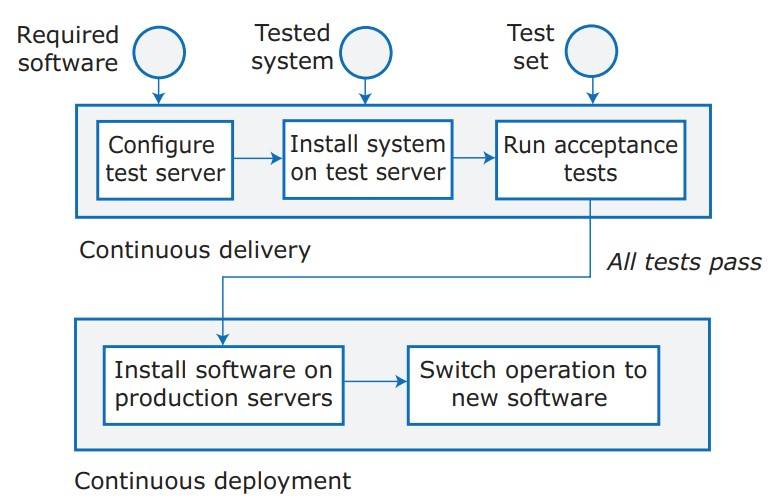
\includegraphics[scale=.5]{img/m3_43}
		\caption{Continuous delivery and deployment}
	\end{figure}
\end{frame}
\begin{frame}{DevOps automation}
	\begin{figure}
		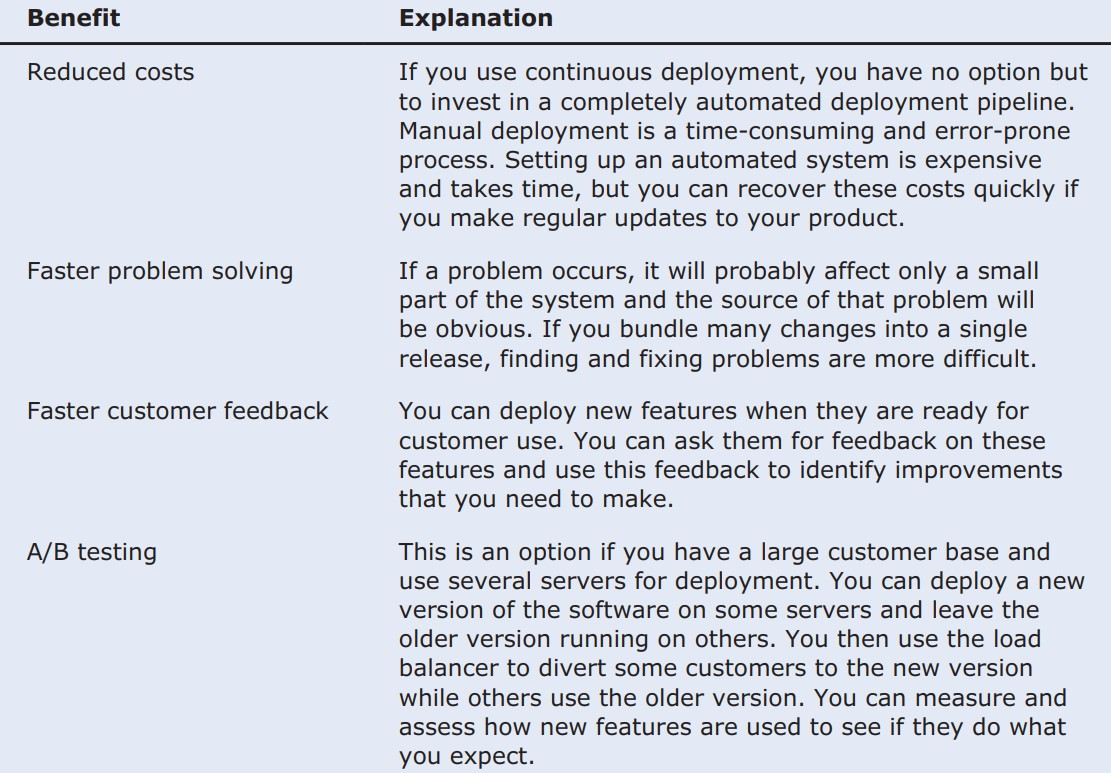
\includegraphics[scale=.43]{img/m3_45}
		\caption{Benefits of continuous deployment}
	\end{figure}
\end{frame}
\begin{frame}{DevOps automation}
	\textbf{Infrastructure as code}
	\begin{itemize}
		\item \textbf{In an enterprise environment}, there are usually many \textbf{different physical or virtual servers} (web servers, database servers, file servers, etc.) \textbf{that do different things.} These \textbf{have different configurations} and run different software packages. 
		\item It is therefore \textbf{difficult to keep track of the software installed on each machine.}
		\item The idea of\textbf{ infrastructure as code was proposed as a way to address this problem}. Rather than manually updating the software on a company’s servers, \textbf{the process can be automated using a model of the infrastructure written in a machine-processable language. }
		\item \textbf{Configuration management (CM) tools }such as Puppet and Chef \textbf{can automatically install software and services on servers according to the infrastructure definition}
		
	\end{itemize}
\end{frame}
\begin{frame}{DevOps automation}
	\begin{figure}
		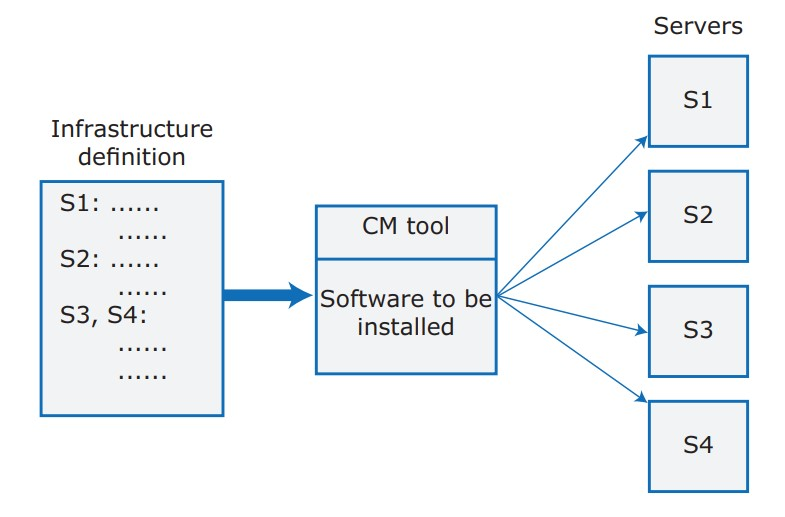
\includegraphics[scale=.5]{img/m3_44}
		\caption{Infrastructure as code}
	\end{figure}
\end{frame}
\begin{frame}{DevOps automation}
	\begin{figure}
		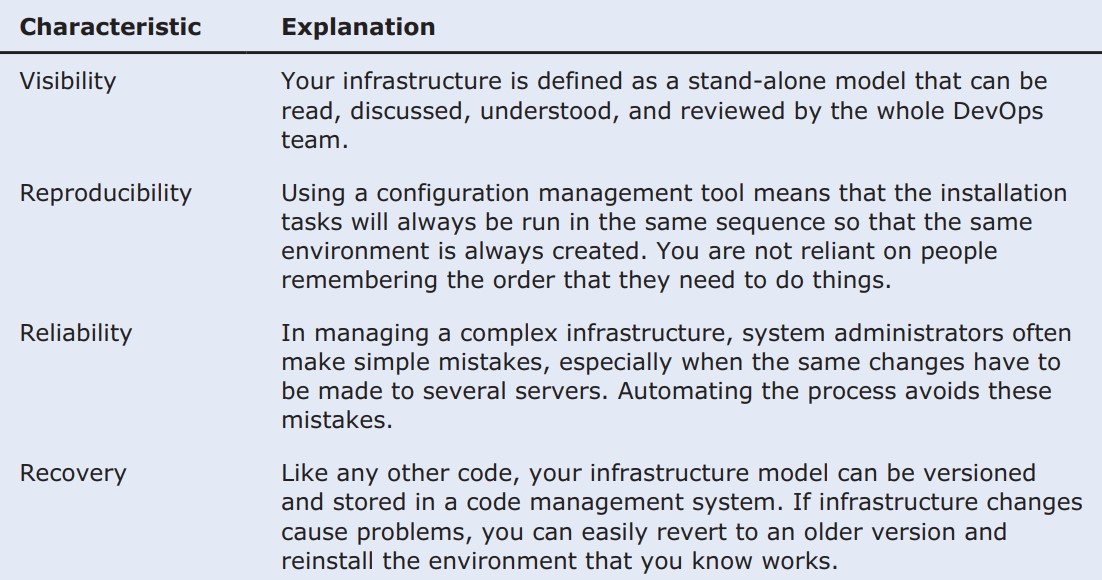
\includegraphics[scale=.43]{img/m3_46}
		\caption{Characteristics of infrastructure as code}
	\end{figure}
\end{frame}
\section{Software Evolution}
\begin{frame}{Software Evolution}
	\textbf{Software Evolution}
	\begin{itemize}
		\item Organisations have huge investments in their 
		software systems - they are critical business 
		assets.
		\item To maintain the value of these assets to the 
		business, they must be changed and updated.
		\item The majority of the software budget in large 
		companies is devoted to changing and 
		evolving existing software rather than 
		developing new software.
	\end{itemize}
\end{frame}
\begin{frame}{Software Evolution}
	\begin{figure}
	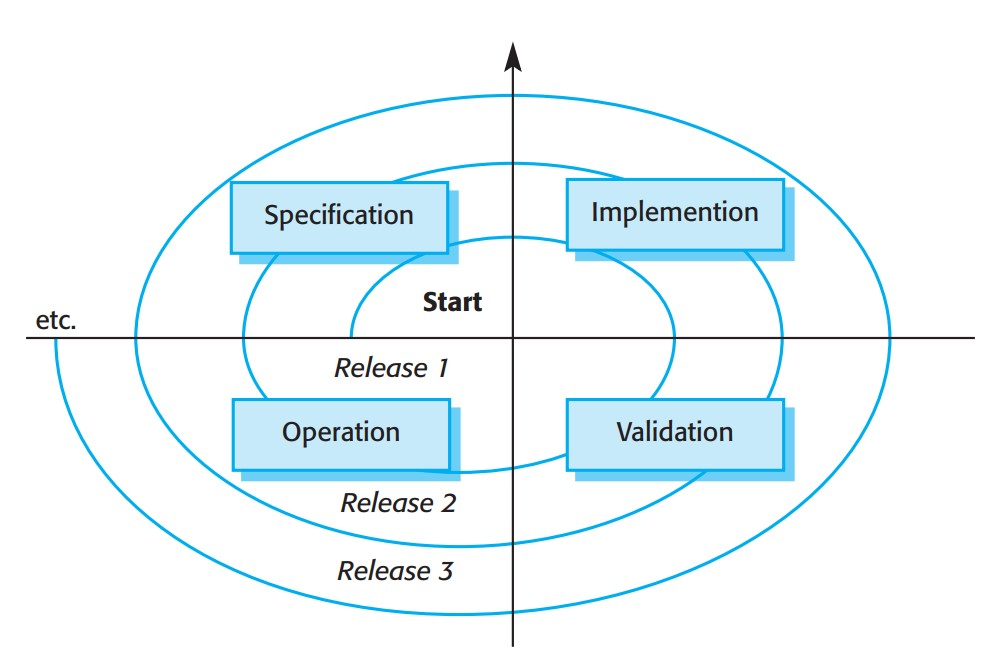
\includegraphics[scale=.43]{img/m3_47}
	\caption{A spiral 
		model of development 
		and evolution }
\end{figure}
\end{frame}
\begin{frame}{Software Evolution}
	\begin{itemize}
		\item Software engineering is a spiral process with requirements, design, implementation, and testing going on throughout the lifetime of the system.
		\item You start by creating release1 of the system.
		\item Once  delivered, changes are proposed, and the development of release2 starts almost immediately.
		\item In fact, the need for evolution may become obvious even before the system is deployed, so later releases of the software may start development before the current version has even been released.
		
	\end{itemize}
\end{frame}
\begin{frame}{Software Evolution}
	\begin{figure}
		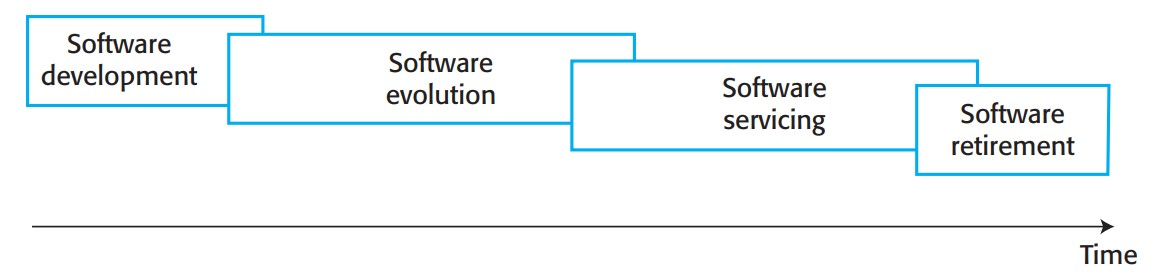
\includegraphics[scale=.43]{img/m3_48}
		\caption{Evolution 
			and servicing 
		}
	\end{figure}
\begin{itemize}
	\item Alternative view of the software evolution life cycle for business systems
	\item In this model, they distinguish between evolution and servicing. 
	\item \textbf{Evolution }is the phase in which significant changes to the software architecture and functionality are made.
	\item During \textbf{servicing}, the only changes that are made are relatively small but essential changes. These phases overlap with each other, as shown in Figure 
	
\end{itemize}
\end{frame}
\begin{frame}{Software Evolution}
\textbf{Evolution processes }
\begin{itemize}
	\item Software evolution processes depend on
	\begin{itemize}
		\item the type of software being mainted.
		\item the development processses used
		\item the skills and experience of the people involved.
	\end{itemize}
\item Proposal for change are the driver for system evolution.
\begin{itemize}
	\item Should be linked with components that are affected by the change, thus allowing the cost and impact of the change to be estimated.
\end{itemize}
\item Change identification and evolution continues throughout the system lifetime
\end{itemize}
\end{frame}
\begin{frame}{Software Evolution}
	\begin{figure}
	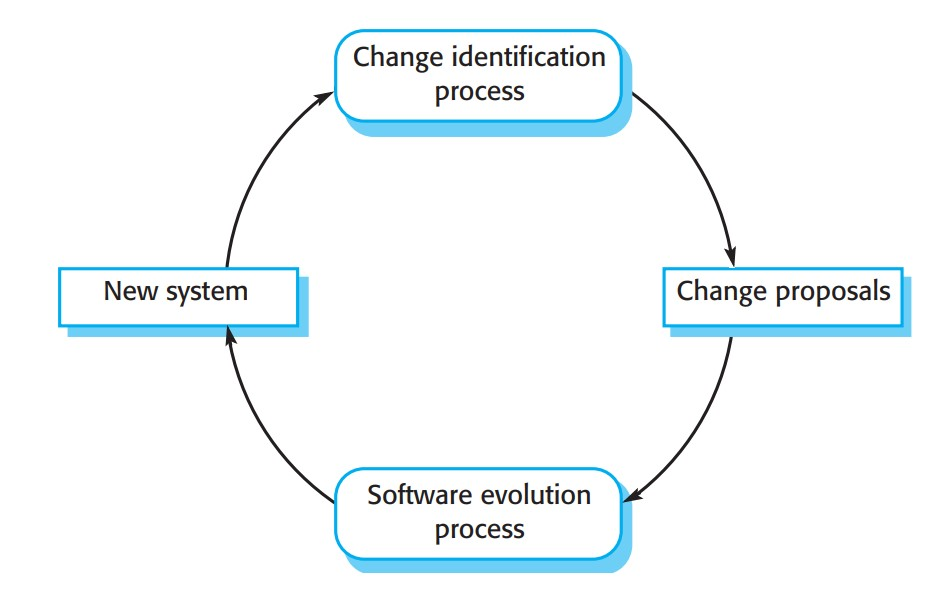
\includegraphics[scale=.43]{img/m3_49}
	\caption{Change 
		identification and 
		evolution processes  }
\end{figure}
\end{frame}
\begin{frame}{Software Evolution}
	\begin{figure}
		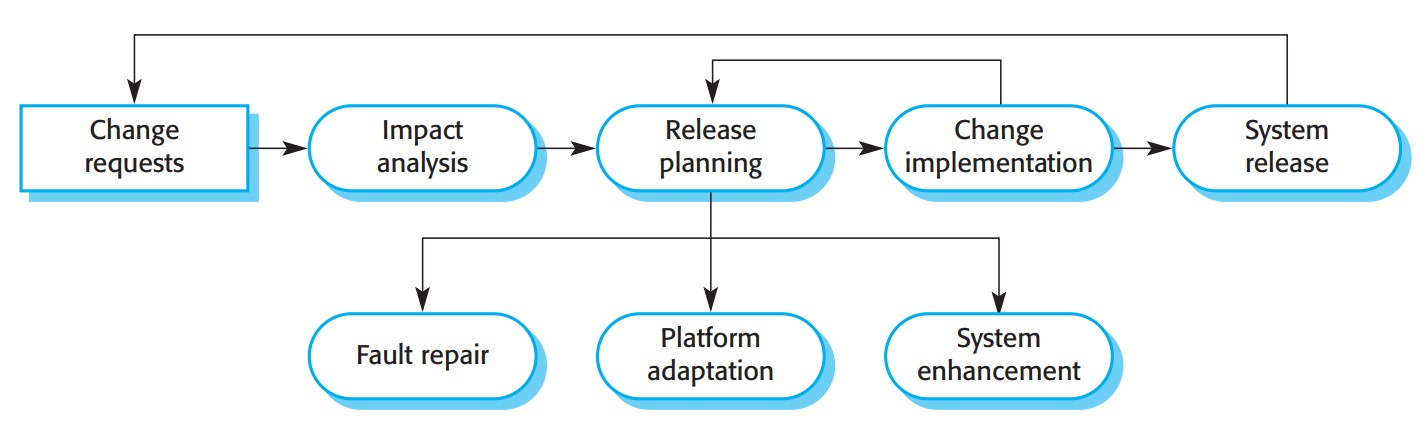
\includegraphics[scale=.4]{img/m3_50}
		\caption{A general 
			model of the software 
			evolution process }
	\end{figure}
\end{frame}
\begin{frame}{Software Evolution}
\begin{itemize}
	\item The process includes the fundamental activities of change analysis, release planning, system implementation, and releasing a system to customers. 
\item The cost and impact of these changes are assessed to see how much of the system is affected by the change and how much it might cost to 
	implement the change. 
\item If the proposed changes are accepted, a new release of the system is planned. 
	\item During release planning, all proposed changes (fault repair, adaptation, and new functionality) are considered.
	\item A decision is then made on which changes to implement in the next version of the system. 
	\item The changes are implemented and validated, and a new version of the system is released. The process then iterates with a new set of changes 
	proposed for the next release. 
\end{itemize}
\end{frame}
\begin{frame}{Software maintenance}
\textbf{Software maintenance}
\begin{itemize}
	\item Software maintenance is the general \textbf{process of changing a system after it has been delivered. }
	\item The term is usually applied to custom software, where separate development groups are involved 
	before and after delivery.
	\item The changes made to the software \textbf{may be simple changes to correct coding errors, more extensive 
		changes to correct design errors, or significant enhancements to correct specification errors or to 
		accommodate new requirements.}

\end{itemize}
\end{frame}
\begin{frame}{Software maintenance}
	\textbf{Types of maintenance}
	\begin{itemize}
		\item \textbf{Fault repairs} to fix bugs and vulnerabilities. Coding errors are usually relatively cheap to correct; design 
		errors are more expensive because they may involve rewriting several program components. 
		Requirements errors are the most expensive to repair because extensive system redesign may be 
		necessary.
		\item \textbf{Environmental adaptation} to adapt the software to new platforms and environments. This type of 
		maintenance is required when some aspect of a system’s environment, such as the hardware, the 
		platform operating system, or other support software, changes. Application systems may have to be 
		modified to cope with these environmental changes.
		\item \textbf{Functionality addition} to add new features and to support new requirements. This type of maintenance 
		is necessary when system requirements change in response to organizational or business change. The 
		scale of the changes required to the software is often much greater than for the other types of 
		maintenance
	\end{itemize}
\end{frame}
\begin{frame}{Software maintenance}
	\textbf{Two important term}
	\begin{itemize}
		\item Maintenance Prediction
		\item Change Prediction
	\end{itemize}
\end{frame}
\begin{frame}{Software maintenance}
	\textbf{Maintenance Prediction:}
	\begin{itemize}
		\item Maintenance prediction \textbf{is concerned with trying to assess the changes that may 
			be required in a software system }and with \textbf{identifying those parts of the system that are likely to be the 
			most expensive to change.}

	\end{itemize}
\end{frame}
\begin{frame}{Software maintenance}
	\textbf{Change Prediction:}
	\begin{itemize}
		\item \textbf{Predicting the number of change requests for a system requires an understanding of the relationship 
			between the system and its external environment.}
		\item Some systems have a very \textbf{complex relationship }
		with their external environment, and changes to that environment inevitably \textbf{result in changes to the 
			system. }
		\item To evaluate the relationships between a system and its environment, you should look at:
		\begin{itemize}
			\item The number and complexity of system interfaces
			\item The number of inherently volatile system requirements
			\item The business processes in which the system is used
		\end{itemize}
	\end{itemize}
\end{frame}
\begin{frame}{Software maintenance}
	\textbf{Software Reengineering }
	\begin{itemize}
		\item Reengineering may \textbf{involve redocumenting the system, refactoring the system architecture, translating 
			programs to a modern programming language, or modifying and updating the structure and values of the system’s data}.
		\item The functionality of the software is not changed, and, normally, you should try to 
		avoid making major changes to the system architecture.

		
	\end{itemize}
\end{frame}
\begin{frame}{Software maintenance}
	\textbf{Refactoring}
	\begin{itemize}
		\item Refactoring is the process of \textbf{making improvements to a program to slow down degradation through 
			change. }
		\item It means \textbf{modifying a program to improve its structure, reduce its complexity, }or make it easier to 
		understand.
		\item Refactoring is sometimes considered to be limited to object-oriented development, but the principles 
		can in fact be applied to any development approach. 
		\item \textbf{When you refactor a program, you should not add functionality but rather should concentrate on 
			program improvement. }
		\item You can therefore think of refactoring as \textbf{“preventative maintenance” that reduces the problems of 
			future change.}
		\item Refactoring is a continuous process of improvement throughout the development and evolution 
		process. It is intended to avoid the structure and code degradation that increases the costs and 
		difficulties of maintaining a system
	\end{itemize}
\end{frame}
\end{document}